% Options for packages loaded elsewhere
\PassOptionsToPackage{unicode}{hyperref}
\PassOptionsToPackage{hyphens}{url}
\PassOptionsToPackage{dvipsnames,svgnames,x11names}{xcolor}
%
\documentclass[
  11pt,
]{article}
\usepackage{amsmath,amssymb}
\usepackage{lmodern}
\usepackage{iftex}
\ifPDFTeX
  \usepackage[T1]{fontenc}
  \usepackage[utf8]{inputenc}
  \usepackage{textcomp} % provide euro and other symbols
\else % if luatex or xetex
  \usepackage{unicode-math}
  \defaultfontfeatures{Scale=MatchLowercase}
  \defaultfontfeatures[\rmfamily]{Ligatures=TeX,Scale=1}
\fi
% Use upquote if available, for straight quotes in verbatim environments
\IfFileExists{upquote.sty}{\usepackage{upquote}}{}
\IfFileExists{microtype.sty}{% use microtype if available
  \usepackage[]{microtype}
  \UseMicrotypeSet[protrusion]{basicmath} % disable protrusion for tt fonts
}{}
\makeatletter
\@ifundefined{KOMAClassName}{% if non-KOMA class
  \IfFileExists{parskip.sty}{%
    \usepackage{parskip}
  }{% else
    \setlength{\parindent}{0pt}
    \setlength{\parskip}{6pt plus 2pt minus 1pt}}
}{% if KOMA class
  \KOMAoptions{parskip=half}}
\makeatother
\usepackage{xcolor}
\IfFileExists{xurl.sty}{\usepackage{xurl}}{} % add URL line breaks if available
\IfFileExists{bookmark.sty}{\usepackage{bookmark}}{\usepackage{hyperref}}
\hypersetup{
  pdftitle={Energy-Aware Ventilation \& Climate Control},
  pdfauthor={Example team: A. Andersson \& B. Berg},
  colorlinks=true,
  linkcolor={RoyalBlue},
  filecolor={Maroon},
  citecolor={Blue},
  urlcolor={Blue},
  pdfcreator={LaTeX via pandoc}}
\urlstyle{same} % disable monospaced font for URLs
\usepackage[a4paper,margin=2.4cm]{geometry}
\usepackage{color}
\usepackage{fancyvrb}
\newcommand{\VerbBar}{|}
\newcommand{\VERB}{\Verb[commandchars=\\\{\}]}
\DefineVerbatimEnvironment{Highlighting}{Verbatim}{commandchars=\\\{\}}
% Add ',fontsize=\small' for more characters per line
\newenvironment{Shaded}{}{}
\newcommand{\AlertTok}[1]{\textcolor[rgb]{1.00,0.00,0.00}{\textbf{#1}}}
\newcommand{\AnnotationTok}[1]{\textcolor[rgb]{0.38,0.63,0.69}{\textbf{\textit{#1}}}}
\newcommand{\AttributeTok}[1]{\textcolor[rgb]{0.49,0.56,0.16}{#1}}
\newcommand{\BaseNTok}[1]{\textcolor[rgb]{0.25,0.63,0.44}{#1}}
\newcommand{\BuiltInTok}[1]{\textcolor[rgb]{0.00,0.50,0.00}{#1}}
\newcommand{\CharTok}[1]{\textcolor[rgb]{0.25,0.44,0.63}{#1}}
\newcommand{\CommentTok}[1]{\textcolor[rgb]{0.38,0.63,0.69}{\textit{#1}}}
\newcommand{\CommentVarTok}[1]{\textcolor[rgb]{0.38,0.63,0.69}{\textbf{\textit{#1}}}}
\newcommand{\ConstantTok}[1]{\textcolor[rgb]{0.53,0.00,0.00}{#1}}
\newcommand{\ControlFlowTok}[1]{\textcolor[rgb]{0.00,0.44,0.13}{\textbf{#1}}}
\newcommand{\DataTypeTok}[1]{\textcolor[rgb]{0.56,0.13,0.00}{#1}}
\newcommand{\DecValTok}[1]{\textcolor[rgb]{0.25,0.63,0.44}{#1}}
\newcommand{\DocumentationTok}[1]{\textcolor[rgb]{0.73,0.13,0.13}{\textit{#1}}}
\newcommand{\ErrorTok}[1]{\textcolor[rgb]{1.00,0.00,0.00}{\textbf{#1}}}
\newcommand{\ExtensionTok}[1]{#1}
\newcommand{\FloatTok}[1]{\textcolor[rgb]{0.25,0.63,0.44}{#1}}
\newcommand{\FunctionTok}[1]{\textcolor[rgb]{0.02,0.16,0.49}{#1}}
\newcommand{\ImportTok}[1]{\textcolor[rgb]{0.00,0.50,0.00}{\textbf{#1}}}
\newcommand{\InformationTok}[1]{\textcolor[rgb]{0.38,0.63,0.69}{\textbf{\textit{#1}}}}
\newcommand{\KeywordTok}[1]{\textcolor[rgb]{0.00,0.44,0.13}{\textbf{#1}}}
\newcommand{\NormalTok}[1]{#1}
\newcommand{\OperatorTok}[1]{\textcolor[rgb]{0.40,0.40,0.40}{#1}}
\newcommand{\OtherTok}[1]{\textcolor[rgb]{0.00,0.44,0.13}{#1}}
\newcommand{\PreprocessorTok}[1]{\textcolor[rgb]{0.74,0.48,0.00}{#1}}
\newcommand{\RegionMarkerTok}[1]{#1}
\newcommand{\SpecialCharTok}[1]{\textcolor[rgb]{0.25,0.44,0.63}{#1}}
\newcommand{\SpecialStringTok}[1]{\textcolor[rgb]{0.73,0.40,0.53}{#1}}
\newcommand{\StringTok}[1]{\textcolor[rgb]{0.25,0.44,0.63}{#1}}
\newcommand{\VariableTok}[1]{\textcolor[rgb]{0.10,0.09,0.49}{#1}}
\newcommand{\VerbatimStringTok}[1]{\textcolor[rgb]{0.25,0.44,0.63}{#1}}
\newcommand{\WarningTok}[1]{\textcolor[rgb]{0.38,0.63,0.69}{\textbf{\textit{#1}}}}
\usepackage{longtable,booktabs,array}
\usepackage{calc} % for calculating minipage widths
% Correct order of tables after \paragraph or \subparagraph
\usepackage{etoolbox}
\makeatletter
\patchcmd\longtable{\par}{\if@noskipsec\mbox{}\fi\par}{}{}
\makeatother
% Allow footnotes in longtable head/foot
\IfFileExists{footnotehyper.sty}{\usepackage{footnotehyper}}{\usepackage{footnote}}
\makesavenoteenv{longtable}
\usepackage{graphicx}
\makeatletter
\def\maxwidth{\ifdim\Gin@nat@width>\linewidth\linewidth\else\Gin@nat@width\fi}
\def\maxheight{\ifdim\Gin@nat@height>\textheight\textheight\else\Gin@nat@height\fi}
\makeatother
% Scale images if necessary, so that they will not overflow the page
% margins by default, and it is still possible to overwrite the defaults
% using explicit options in \includegraphics[width, height, ...]{}
\setkeys{Gin}{width=\maxwidth,height=\maxheight,keepaspectratio}
% Set default figure placement to htbp
\makeatletter
\def\fps@figure{htbp}
\makeatother
\setlength{\emergencystretch}{3em} % prevent overfull lines
\providecommand{\tightlist}{%
  \setlength{\itemsep}{0pt}\setlength{\parskip}{0pt}}
\setcounter{secnumdepth}{-\maxdimen} % remove section numbering
\usepackage{newunicodechar}
\usepackage{textcomp}
\usepackage{amssymb}
\newunicodechar{°}{\textdegree}
\newunicodechar{₂}{\textsubscript{2}}
\newunicodechar{→}{\ensuremath{\rightarrow}}
\newunicodechar{≤}{\ensuremath{\leq}}
\newunicodechar{≥}{\ensuremath{\geq}}
\newunicodechar{≈}{\ensuremath{\approx}}
\newunicodechar{✓}{\ensuremath{\checkmark}}
\newunicodechar{–}{--}
\newunicodechar{—}{---}
\usepackage{etoolbox}
\AtBeginEnvironment{longtable}{\footnotesize}
\AtBeginEnvironment{tabular}{\footnotesize}
\usepackage{fancyhdr}
\pagestyle{fancy}\fancyhf{}
\rhead{\small D7065E\,--\,Architecture Document}
\lhead{\small Example: Energy-Aware Ventilation Control}
\cfoot{\thepage}
\renewcommand{\headrulewidth}{0.4pt}
\usepackage{titlesec}
\titleformat{\section}{\Large\bfseries}{\thesection}{0.6em}{}
\titleformat{\subsection}{\large\bfseries}{\thesubsection}{0.5em}{}
\usepackage{microtype}
\usepackage{pgfplots}
\pgfplotsset{compat=1.16}
\setlength{\emergencystretch}{2em}
\ifLuaTeX
  \usepackage{selnolig}  % disable illegal ligatures
\fi

\title{Energy-Aware Ventilation \& Climate Control}
\usepackage{etoolbox}
\makeatletter
\providecommand{\subtitle}[1]{% add subtitle to \maketitle
  \apptocmd{\@title}{\par {\large #1 \par}}{}{}
}
\makeatother
\subtitle{D7065E, Architecture Document (worked example, targeting
grade 5)}
\author{Example team: A. Andersson \& B. Berg}
\date{}

\begin{document}

{\setlength{\fboxsep}{7pt}\setlength{\fboxrule}{0.6pt}%
\begin{center}
\fbox{\fbox{\parbox{0.88\linewidth}{%
\textbf{Read this first.} A worked example of a final architecture
document (use case: energy-aware ventilation \& climate control), written
to the \textbf{grade-5 standard}, choices justified against
alternatives, requirements traced to validation, the system reasoned
about as a whole, and evaluation backed by measured evidence and honest
critique. It is \emph{not} a recommended or canonical architecture:
simpler or more complex solutions can earn the highest grade if equally
well justified, tested, and evaluated. \textbf{Copying the architecture, technologies, or text does not help}, in the oral examination each author must explain and defend the design decisions independently.%
}}}
\end{center}}

\vspace{1.2em}

\begin{center}
{\LARGE Energy-Aware Ventilation \& Climate Control\par}
\vspace{0.5em}
{\large D7065E, Architecture Document (worked example, targeting grade 5)\par}
\vspace{1em}
{Example team: A. Andersson \& B. Berg\par}
\end{center}

\vspace{1.2em}

{
\hypersetup{linkcolor=black}
\setcounter{tocdepth}{3}
\tableofcontents
}

\hypertarget{summary}{%
\section{1. Summary}\label{summary}}

This system keeps the rooms of a building comfortable and healthy while
using as little energy as possible. It senses temperature, CO₂, and
occupancy per room; an \textbf{autonomous service} decides how much to
ventilate and heat each zone; and actuators drive the HVAC setpoint and
ventilation dampers. The building itself, its rooms, sensors,
actuators, and 3D view, is provided by \textbf{BuildSim}, which holds
the shared building state; this project provides the physics, the intelligence, and
the control around it. The guiding principle is simple and is the thread
through every later decision: \textbf{ventilate and heat where and when
people actually are, and ease off everywhere else.}

\begin{longtable}[]{@{}
  >{\raggedright\arraybackslash}p{(\columnwidth - 2\tabcolsep) * \real{0.5000}}
  >{\raggedright\arraybackslash}p{(\columnwidth - 2\tabcolsep) * \real{0.5000}}@{}}
\toprule
\begin{minipage}[b]{\linewidth}\raggedright
Field
\end{minipage} & \begin{minipage}[b]{\linewidth}\raggedright
Value
\end{minipage} \\
\midrule
\endhead
\textbf{Project title} & Energy-Aware Ventilation \& Climate Control \\
\textbf{Team members} & A. Andersson, B. Berg \\
\textbf{Use case} & Indoor air quality + thermal comfort at minimum
energy \\
\textbf{Repository} &
\texttt{github.com/example-team/d7065e-ventilation} \\
\textbf{Version / date} & v1.6 / 2026-09-24 \\
\bottomrule
\end{longtable}

\textbf{Changes since the proposal.} Two design changes were made
\emph{because the evidence demanded it}, which is the point of building
iteratively. First, the proposal sent readings straight to the
autonomous service over REST; once a dashboard and historical storage
also needed the same readings, the design moved to an \textbf{MQTT broker} so
each sensor publishes once and every consumer subscribes independently.
Second, the proposal planned a machine-learning occupancy predictor; on
two weeks of simulated data it gave no measurable benefit over a
transparent \textbf{rolling estimate with a time-of-day prior}, so the autonomous service was kept rule-based and spent the time saved on
data-quality handling and testing. Both decisions are revisited in
Section 7.

\hypertarget{use-case-and-building-context-buildsim}{%
\section{2. Use case and building context
(BuildSim)}\label{use-case-and-building-context-buildsim}}

\textbf{The building.} The system controls a multi-room office floor
modelled in \textbf{BuildSim}. BuildSim is the \emph{shared state} of
the cyber-physical system: it owns the building model (rooms, levels,
equipment), exposes a \textbf{REST API} to register devices and to read
and write their state, and streams live state to a \textbf{3D web
viewer} over WebSocket. BuildSim is not modified; it is instrumented.
This separation is deliberate, it is exactly the seam between the
\emph{physical half} of a CPS (the building, behind BuildSim's API) and
the \emph{cyber half} (the project's processes), and keeping that seam clean is
what would let the same software later drive a real building instead of
a simulated one.

\textbf{How the system connects to BuildSim.} Each of the project's processes
talks to BuildSim through its API, and nothing else touches the building
state directly:

\begin{itemize}
\tightlist
\item
  \textbf{Sensor processes} read their sensor's current value from
  BuildSim (\texttt{GET\ /api/sensors/\{id\}}) and publish it to the MQTT broker, so the pipeline and autonomous service can consume it. They
  emulate IoT devices that observe the environment and report it, they
  do not generate the values themselves.
\item
  \textbf{Actuator processes} receive commands from the autonomous
  service and apply them to BuildSim
  (\texttt{PUT\ /api/actuators/\{id\}/state}); BuildSim is the single
  source of truth for actuator state.
\item
  \textbf{The physical simulator} (Section 6) interacts \emph{only} with
  BuildSim: it reads the current actuator state, advances the room
  physics, and writes the resulting sensor values back into BuildSim
  (\texttt{PUT\ /api/sensors/\{id\}/value}), this is what closes the
  feedback loop.
\item
  \textbf{The dashboard} subscribes to BuildSim's WebSocket session API
  to highlight rooms and overlay the system's decisions on the 3D view.
\end{itemize}

\textbf{Actors.} The \textbf{building manager} monitors the system and
may override it; \textbf{occupants} influence it only by being present,
which the occupancy sensors detect. Neither actor is on the control path, the loop runs autonomously.

\textbf{The scenario the demo tells.} On a weekday morning, occupants
arrive and a meeting fills room A2306. Body heat and exhaled CO₂ push
temperature and CO₂ up. The autonomous service detects the rising CO₂
and the occupancy, increases ventilation in that zone, and holds the
temperature in band, then, when the room empties, it falls back to a
low-energy setback. Meanwhile unoccupied rooms are never heated or
ventilated beyond the regulatory minimum. The same loop runs in every
room, every cycle.

\textbf{Why it matters.} Buildings are among the largest energy
consumers in Sweden, and ventilation and heating dominate that load. A
controller that follows occupancy rather than the clock saves energy
\emph{and} improves air quality, but only if it is fast enough to react,
robust enough to survive a failed sensor, and trustworthy enough to
leave running. Those three concerns, latency, resilience, trust, drive the requirements in Section 3.

\textbf{Where this system sits.} Ventilation control is only one of
several systems that run on the same building. The C4 \emph{System
Landscape} below shows the bigger picture, fire detection, security,
energy management, and ours are each built on BuildSim and overseen by
the facilities team. This report designs the highlighted system.

\begin{center}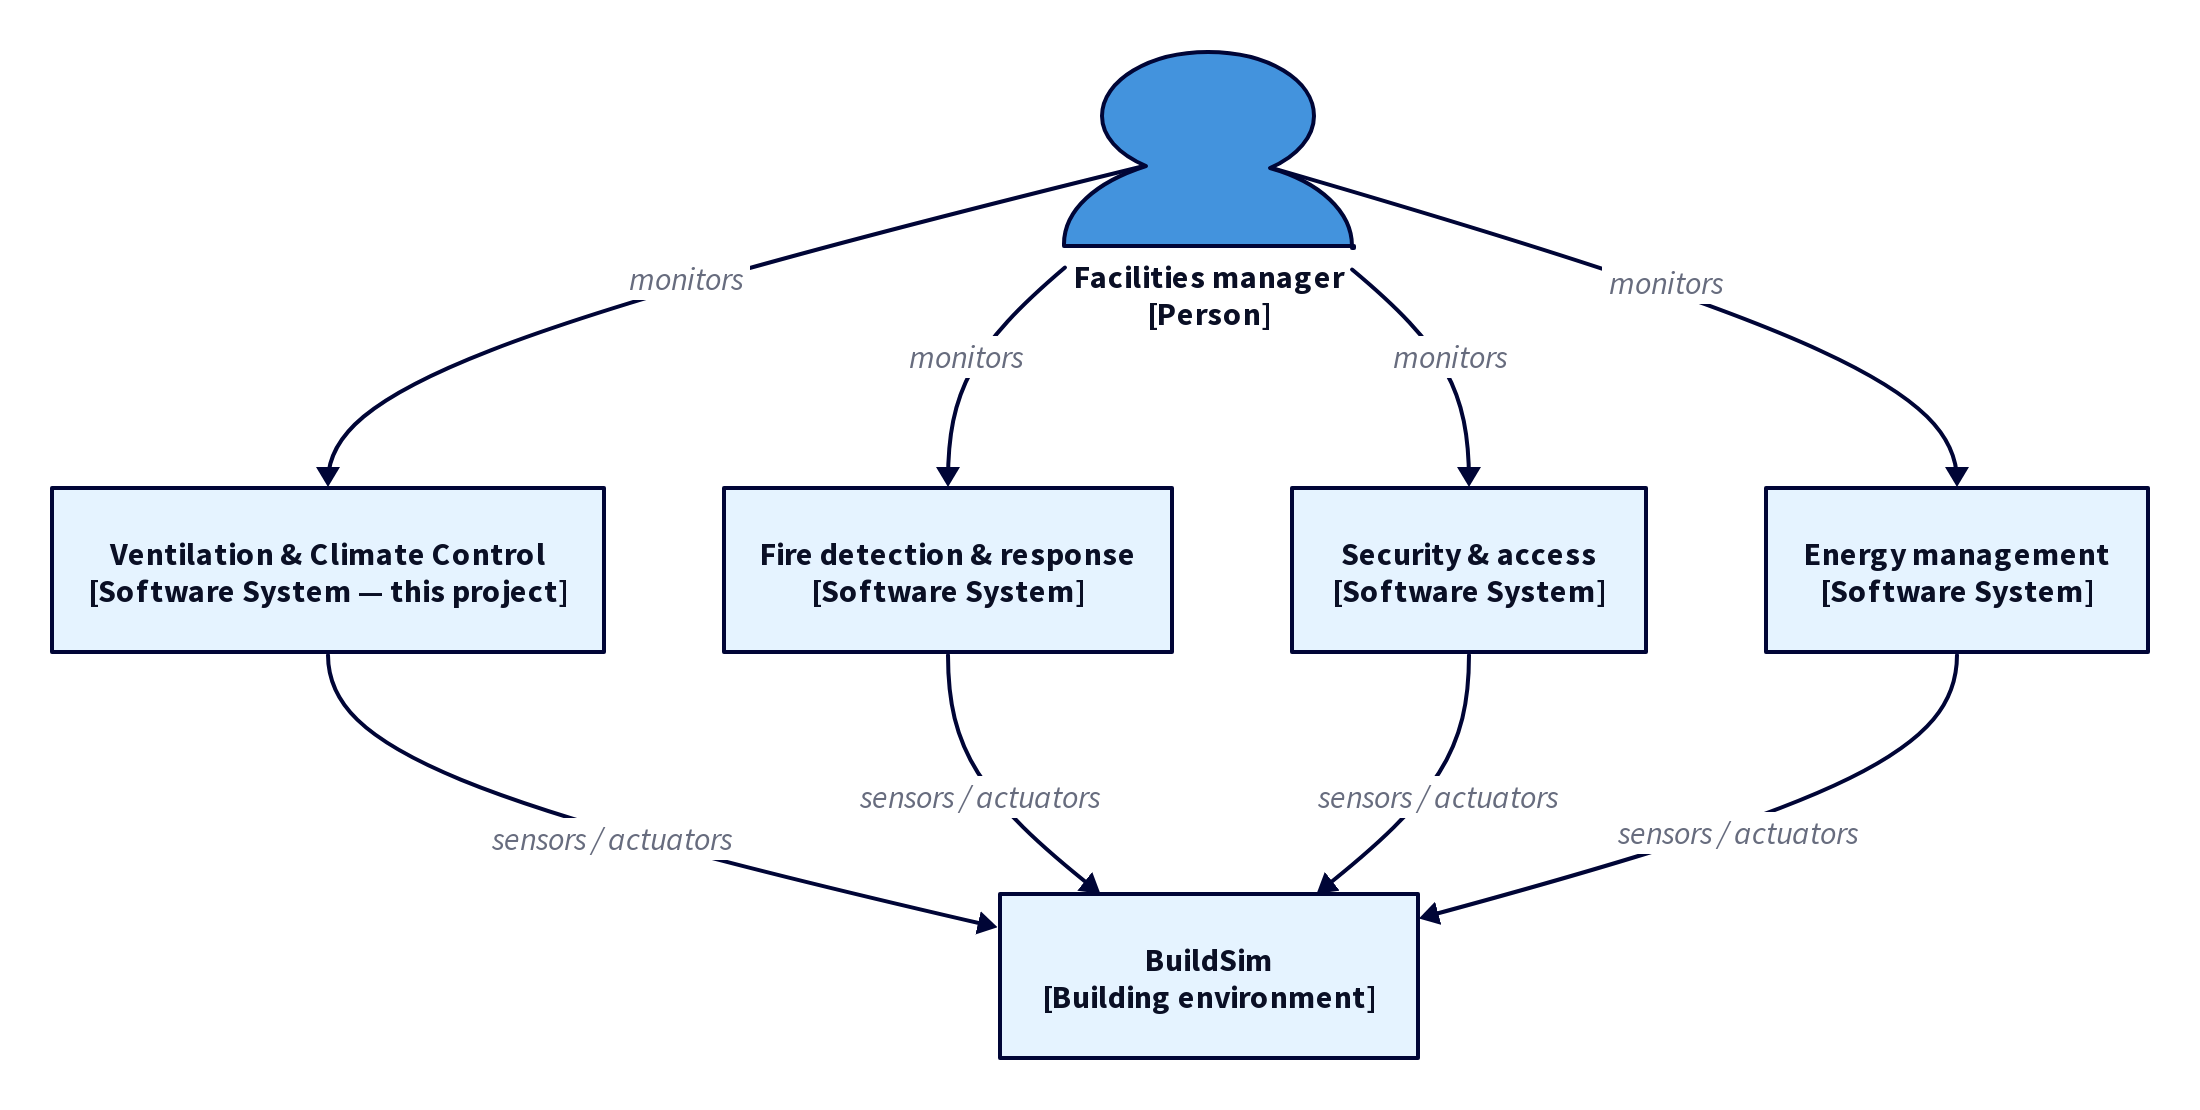
\includegraphics[width=0.55\textwidth]{figures/landscape.png}\end{center}

\noindent{\footnotesize\emph{C4 System Landscape. Several independent
building systems, each on BuildSim; the highlighted system is the one
this report designs.}}

\hypertarget{requirements}{%
\section{3. Requirements}\label{requirements}}

The requirements below are the root of the MBSE thread: each is a
\textbf{testable} statement with a unique ID, traced to a design element
(Sections 4--9) and a verification (Section 10). Functional requirements
(FR) say what the system does; non-functional requirements (NFR) say how
well; the regulatory requirement (REG) comes from the Swedish Work
Environment Authority's ventilation guidance. Vague requirements cannot
be tested, so every one here is quantified.

\begin{longtable}[]{@{}
  >{\raggedright\arraybackslash}p{(\columnwidth - 10\tabcolsep) * \real{0.0588}}
  >{\raggedright\arraybackslash}p{(\columnwidth - 10\tabcolsep) * \real{0.0882}}
  >{\raggedright\arraybackslash}p{(\columnwidth - 10\tabcolsep) * \real{0.1912}}
  >{\raggedright\arraybackslash}p{(\columnwidth - 10\tabcolsep) * \real{0.1471}}
  >{\raggedright\arraybackslash}p{(\columnwidth - 10\tabcolsep) * \real{0.3235}}
  >{\raggedright\arraybackslash}p{(\columnwidth - 10\tabcolsep) * \real{0.1912}}@{}}
\toprule
\begin{minipage}[b]{\linewidth}\raggedright
ID
\end{minipage} & \begin{minipage}[b]{\linewidth}\raggedright
Type
\end{minipage} & \begin{minipage}[b]{\linewidth}\raggedright
Requirement
\end{minipage} & \begin{minipage}[b]{\linewidth}\raggedright
Priority
\end{minipage} & \begin{minipage}[b]{\linewidth}\raggedright
Acceptance criterion
\end{minipage} & \begin{minipage}[b]{\linewidth}\raggedright
Verified by
\end{minipage} \\
\midrule
\endhead
FR-01 & Functional & Keep an occupied room's CO₂ below 1000 ppm by
ventilating & Must & CO₂ returns below 1000 ppm within 10 min of
exceeding it while occupied & \texttt{test\_co2\_recovery} \\
FR-02 & Functional & Hold occupied rooms within the comfort band 20--24
°C & Must & In band ≥ 90 \% of occupied minutes &
\texttt{test\_comfort\_band} \\
FR-03 & Functional & Set back ventilation and heating in empty rooms &
Must & Fan and setpoint drop within 15 min of a room emptying &
\texttt{test\_setback} \\
NFR-01 & Non-functional & Produce a control decision at least every 60 s
per zone & Must & Median decision interval ≤ 60 s under full load &
\texttt{test\_decision\_interval} \\
NFR-02 & Non-functional & Survive a sensor-process crash without losing
control & Must & A new reading reaches storage within 60 s of a kill &
\texttt{test\_sensor\_recovery} \\
NFR-03 & Non-functional & Avoid actuator thrashing & Should & No
actuator changes state more than once per 5 min &
\texttt{test\_no\_thrashing} \\
NFR-04 & Non-functional & Use less energy than a fixed-schedule baseline
& Should & ≥ 15 \% lower modelled energy over one week &
\texttt{test\_energy\_saving} \\
REG-01 & Regulatory & Maintain a minimum ventilation rate even when
empty & Must & Fan never drops below the configured minimum &
\texttt{test\_min\_ventilation} \\
\bottomrule
\end{longtable}

A deliberate \textbf{tension} runs through these requirements, air
quality and comfort pull ventilation up (FR-01, FR-02), energy pulls it
down (NFR-04), and the regulatory floor (REG-01) sets a hard minimum.
Resolving that tension safely is the whole job of the autonomous
service, and it is why a single threshold rule is not enough.

\textbf{Traceability.} The five architecture viewpoints map onto this
document so nothing is left unverified: \emph{context} (4.1),
\emph{functional/container} (4.2--4.3), \emph{information/data} (6--7),
\emph{behavioural} (8), \emph{deployment} (9). Each requirement names
the design that satisfies it and the test that proves it; the plan in
Section 10 closes the loop.

\hypertarget{architecture}{%
\section{4. Architecture}\label{architecture}}

\hypertarget{context-diagram-c4-level-1}{%
\subsection{4.1 Context diagram (C4 Level
1)}\label{context-diagram-c4-level-1}}

The context view fixes the \textbf{system boundary}: what is ours to
build versus what is outside. The system reads and commands the building
only through BuildSim; the building manager monitors and may override;
occupants are sensed, not connected; and an optional external analysis
service is used only for overnight analysis, never on the control path.

\begin{center}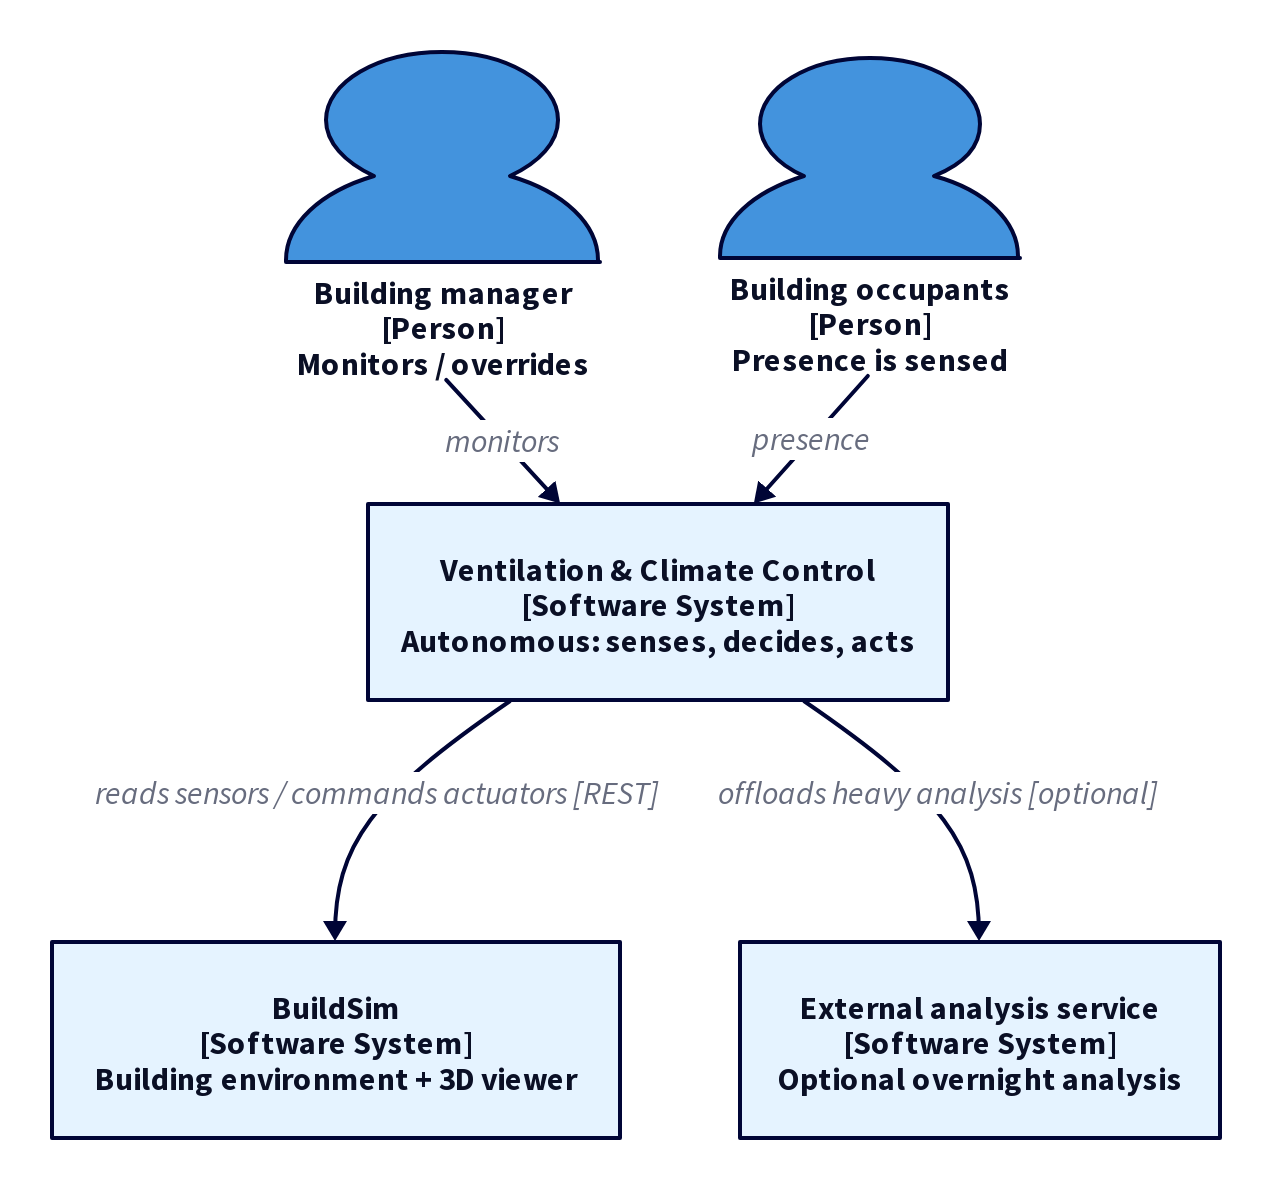
\includegraphics[width=0.64\textwidth]{figures/context.png}\end{center}

\noindent{\footnotesize\emph{C4 System Context (Level 1). Person and software-system elements; the system in scope is highlighted, external systems are grey; every arrow is a directed relationship labelled with its purpose and protocol.}}

\hypertarget{container-diagram-c4-level-2}{%
\subsection{4.2 Container diagram (C4 Level
2)}\label{container-diagram-c4-level-2}}

Each box is one Docker container and one repository folder; the arrows
carry the protocol. \textbf{BuildSim is the environment} and the
system's shared state. The physical simulator interacts \emph{only} with
BuildSim: it reads the current actuator state, advances the room physics,
and writes the resulting sensor values back into BuildSim. The sensor
processes then read those values from BuildSim and publish them onto the
broker; the autonomous service decides and commands the actuator
processes, which write actuator state back to BuildSim. That actuator
change alters the environment the simulator advances next tick, the
closed loop that makes this a cyber-physical system rather than a
dashboard.

\begin{center}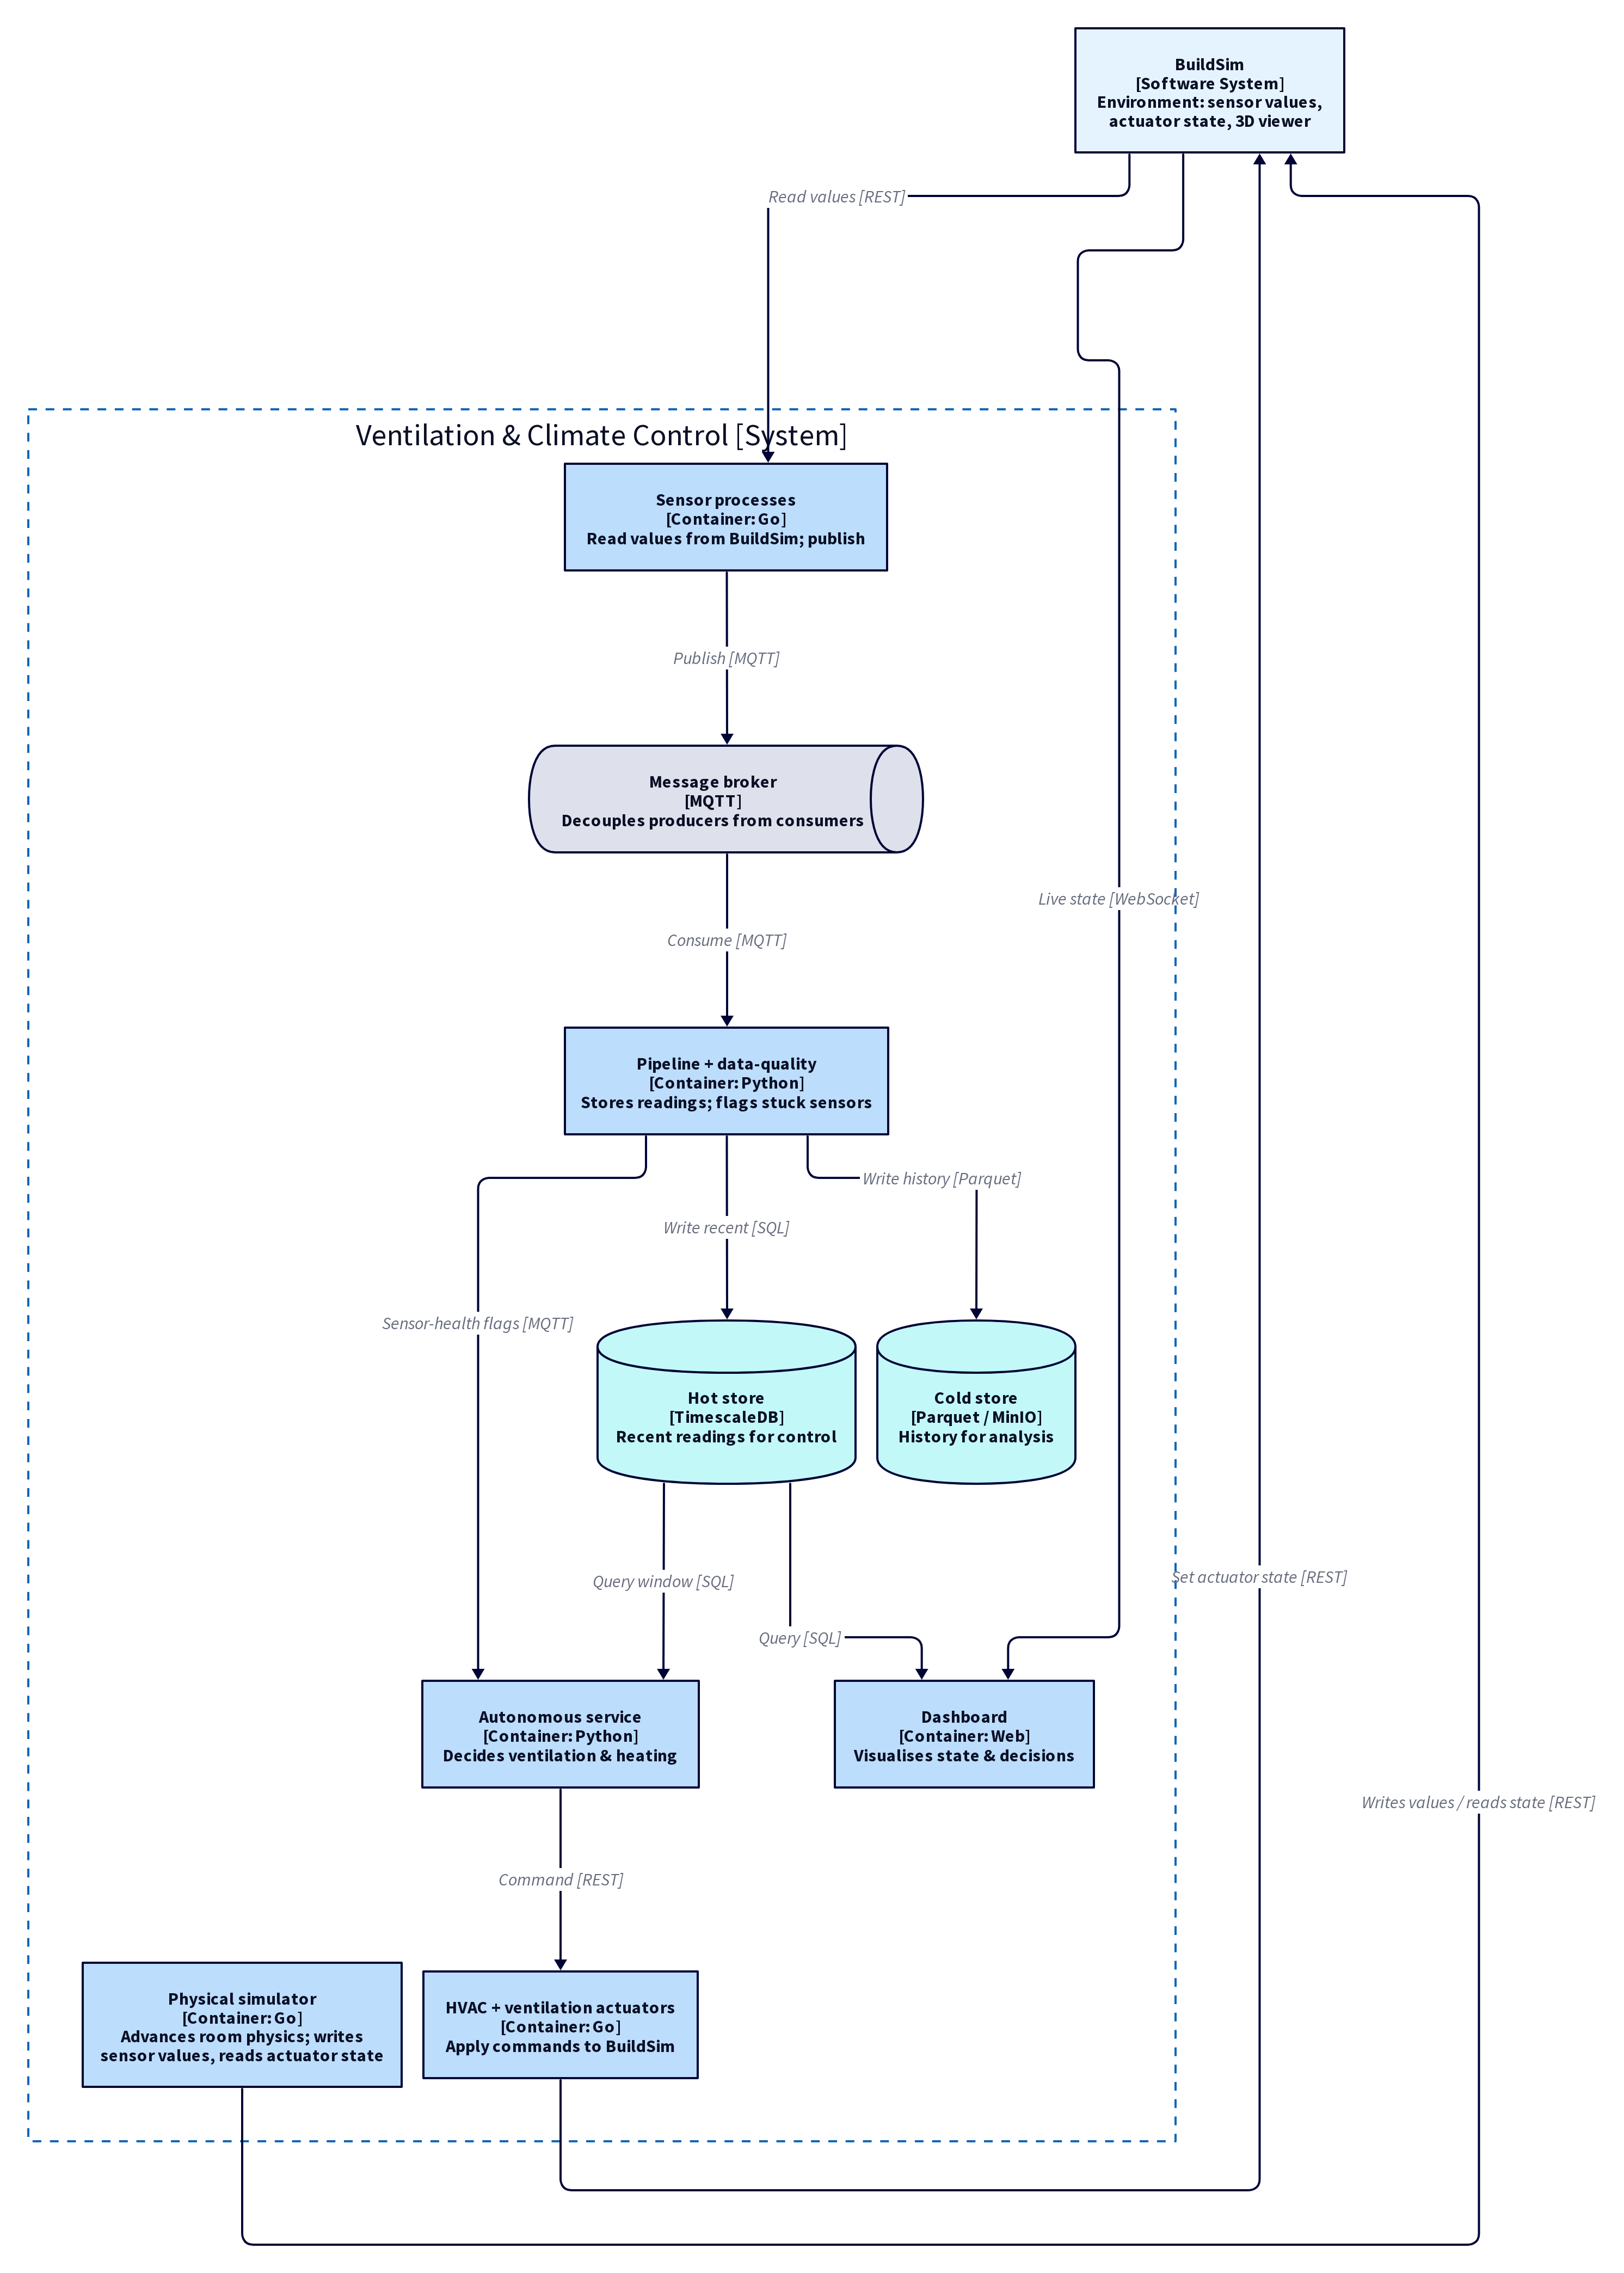
\includegraphics[height=0.9\textheight]{figures/container.png}\end{center}

\noindent{\footnotesize\emph{C4 Container diagram (Level 2). Each container shows its [technology] and responsibility; the in-scope system is the dashed boundary, external systems (BuildSim) are grey; every arrow is a directed relationship labelled with its protocol.}}

\hypertarget{component-responsibilities}{%
\subsection{4.3 Component
responsibilities}\label{component-responsibilities}}

Every container has a single responsibility, the principle that makes
the system testable and lets one part fail without taking down the rest.
The ``reason for separation'' column is where that systems-level
reasoning is made explicit.

\begin{longtable}[]{@{}
  >{\raggedright\arraybackslash}p{(\columnwidth - 8\tabcolsep) * \real{0.1410}}
  >{\raggedright\arraybackslash}p{(\columnwidth - 8\tabcolsep) * \real{0.3333}}
  >{\raggedright\arraybackslash}p{(\columnwidth - 8\tabcolsep) * \real{0.1410}}
  >{\raggedright\arraybackslash}p{(\columnwidth - 8\tabcolsep) * \real{0.0769}}
  >{\raggedright\arraybackslash}p{(\columnwidth - 8\tabcolsep) * \real{0.3077}}@{}}
\toprule
\begin{minipage}[b]{\linewidth}\raggedright
Component
\end{minipage} & \begin{minipage}[b]{\linewidth}\raggedright
Responsibility (one job)
\end{minipage} & \begin{minipage}[b]{\linewidth}\raggedright
Container
\end{minipage} & \begin{minipage}[b]{\linewidth}\raggedright
Tech
\end{minipage} & \begin{minipage}[b]{\linewidth}\raggedright
Reason for separation
\end{minipage} \\
\midrule
\endhead
Temperature sensor & Read simulated temp, publish & \texttt{temp-sensor}
& Go & One per room; independent restart \\
CO₂ sensor & Read simulated CO₂, publish & \texttt{co2-sensor} & Go &
Same lifecycle, different signal \\
Occupancy sensor & Publish presence / count & \texttt{occupancy-sensor}
& Go & Drives both control and features \\
Physical simulator & Compute room physics from actuator state &
\texttt{simulator} & Python & Models the building; closes the loop \\
MQTT broker & Decouple publishers from consumers & \texttt{mosquitto} &
Mosquitto & One source, many consumers \\
Pipeline consumer & Persist readings (hot + cold) & \texttt{pipeline} &
Python & Decouples ingestion from sensing \\
Data-quality monitor & Detect stuck / stale sensors &
\texttt{dq-monitor} & Python & Second technique; protects the
controller \\
Autonomous service & Decide ventilation and heating &
\texttt{control-service} & Python & Decision logic evolves
independently \\
HVAC / vent actuators & Apply commands to BuildSim & \texttt{*-actuator}
& Go & Separate failure domains \\
Dashboard & Visualise state and decisions & \texttt{dashboard} & Web &
Separates presentation from logic \\
\bottomrule
\end{longtable}

\hypertarget{design-decisions-and-justifications}{%
\subsection{4.4 Design decisions and
justifications}\label{design-decisions-and-justifications}}

This table carries most of the architecture grade. Each row states the
option chosen, the alternative genuinely considered, the requirement it
serves, and the trade-off accepted. A decision with no rejected
alternative is only an assumption.

\begin{longtable}[]{@{}
  >{\raggedright\arraybackslash}p{(\columnwidth - 8\tabcolsep) * \real{0.1389}}
  >{\raggedright\arraybackslash}p{(\columnwidth - 8\tabcolsep) * \real{0.1111}}
  >{\raggedright\arraybackslash}p{(\columnwidth - 8\tabcolsep) * \real{0.1944}}
  >{\raggedright\arraybackslash}p{(\columnwidth - 8\tabcolsep) * \real{0.4028}}
  >{\raggedright\arraybackslash}p{(\columnwidth - 8\tabcolsep) * \real{0.1528}}@{}}
\toprule
\begin{minipage}[b]{\linewidth}\raggedright
Decision
\end{minipage} & \begin{minipage}[b]{\linewidth}\raggedright
Chosen
\end{minipage} & \begin{minipage}[b]{\linewidth}\raggedright
Alternatives
\end{minipage} & \begin{minipage}[b]{\linewidth}\raggedright
Justification (requirement)
\end{minipage} & \begin{minipage}[b]{\linewidth}\raggedright
Trade-off
\end{minipage} \\
\midrule
\endhead
Sensor transport & MQTT pub/sub & Direct REST; Kafka & Three consumers
need the same readings; broker buffers if one is down (NFR-02) & A
broker to run and monitor \\
Storage split & TimescaleDB (hot) + Parquet/MinIO (cold) & Single
relational DB; files only & Fast recent-window queries for control,
cheap history for analysis (NFR-01, NFR-04) & Two stores to keep
consistent \\
Control approach & Rule-based + hysteresis + setback & ML controller;
MPC optimiser & Meets the 60 s budget, is verifiable, matched ML on the available data (NFR-01) & Less adaptive than a learned controller \\
Data quality & Dedicated stuck-sensor monitor & Trust raw readings & A
frozen sensor is a safety risk, not just noise (FR-01) & Extra component
and tuning \\
Decomposition & One container per role & Monolith & Fault isolation and
independent restart (NFR-02) & More inter-process communication \\
Heavy analysis & Overnight, on external compute & Real-time, on the laptop &
Keeps the control loop fast; analysis is off the critical path (NFR-01)
& Occupancy prior updates daily, not live \\
\bottomrule
\end{longtable}

\hypertarget{interfaces-and-communication}{%
\section{5. Interfaces and
communication}\label{interfaces-and-communication}}

Three communication patterns are used, each for the job it fits.
\textbf{MQTT pub/sub} carries sensor readings because one sensor feeds
many consumers and the broker buffers if a consumer is briefly down.
\textbf{REST} carries device registration and actuator commands, including every call to BuildSim, because each is a one-to-one
request whose result the caller must confirm. \textbf{WebSocket}
(BuildSim's) pushes live state to the dashboard without polling.
Specifying these precisely is what would let another team rebuild the
system from this section alone.

Every reading is a JSON object with explicit units, so no consumer has
to guess:

\begin{Shaded}
\begin{Highlighting}[]
\FunctionTok{\{}
  \DataTypeTok{"ts"}\FunctionTok{:} \StringTok{"2026{-}09{-}24T09:14:00Z"}\FunctionTok{,}
  \DataTypeTok{"sensor\_id"}\FunctionTok{:} \StringTok{"co2{-}A2306"}\FunctionTok{,}
  \DataTypeTok{"room"}\FunctionTok{:} \StringTok{"A2306"}\FunctionTok{,}
  \DataTypeTok{"type"}\FunctionTok{:} \StringTok{"co2"}\FunctionTok{,}
  \DataTypeTok{"unit"}\FunctionTok{:} \StringTok{"ppm"}\FunctionTok{,}
  \DataTypeTok{"value"}\FunctionTok{:} \DecValTok{612}
\FunctionTok{\}}
\end{Highlighting}
\end{Shaded}

\begin{longtable}[]{@{}
  >{\raggedright\arraybackslash}p{(\columnwidth - 8\tabcolsep) * \real{0.1930}}
  >{\raggedright\arraybackslash}p{(\columnwidth - 8\tabcolsep) * \real{0.1930}}
  >{\raggedright\arraybackslash}p{(\columnwidth - 8\tabcolsep) * \real{0.1754}}
  >{\raggedright\arraybackslash}p{(\columnwidth - 8\tabcolsep) * \real{0.3158}}
  >{\raggedright\arraybackslash}p{(\columnwidth - 8\tabcolsep) * \real{0.1228}}@{}}
\toprule
\begin{minipage}[b]{\linewidth}\raggedright
Interface
\end{minipage} & \begin{minipage}[b]{\linewidth}\raggedright
Direction
\end{minipage} & \begin{minipage}[b]{\linewidth}\raggedright
Protocol
\end{minipage} & \begin{minipage}[b]{\linewidth}\raggedright
Endpoint / topic
\end{minipage} & \begin{minipage}[b]{\linewidth}\raggedright
Notes
\end{minipage} \\
\midrule
\endhead
Simulator → BuildSim & write sensor values & REST &
\texttt{PUT\ /api/sensors/\{id\}/value} & makes the reading visible in
the 3D viewer \\
Sensor ← BuildSim & read value & REST & \texttt{GET\ /api/sensors/\{id\}}
& the sensor samples the environment \\
Sensor → broker & publish & MQTT & \texttt{sensors/\{room\}/\{type\}} &
QoS 1, every 5 s \\
Service → BuildSim & command & REST &
\texttt{PUT\ /api/actuators/\{id\}/state} & 200 ok; 409 if manually
overridden \\
Simulator ← BuildSim & read state & REST & \texttt{GET\ /api/actuators}
& closes the physical loop \\
Service → dashboard & publish & MQTT & \texttt{decisions/\{room\}} &
carries a human-readable reason \\
\bottomrule
\end{longtable}

Each decision message carries a \textbf{reason} string
(e.g.~\texttt{"CO2\ 740ppm\ rising,\ 5\ occupants\ -\textgreater{}\ fan\ level\ 2"})
so that every action is auditable after the fact, a small choice with
a large effect on whether the system can be trusted.

\hypertarget{simulating-the-sensor-values-the-physical-model}{%
\section{6. Simulating the sensor values (the physical
model)}\label{simulating-the-sensor-values-the-physical-model}}

Because BuildSim provides the rooms but not their physics, \textbf{the physical simulator that generates realistic sensor values was built}.
The aim is not a physically perfect model but one with enough structure, trends, daily cycles, and genuine responses to actuator commands, that the autonomous service reacts to meaningful data and the closed
loop actually closes. The simulator reads the current actuator state
from BuildSim each tick (5 s), updates each room's physical state, and
writes the new sensor values back into BuildSim; the sensor processes
then read those values and publish them onto the broker. A \textbf{physics-based} model is used rather than replaying recorded traces,
because the sensor values must respond to the actuators, and that
response to actuation is exactly what the control loop depends on.

\textbf{Occupancy} drives everything else, so it is modelled explicitly, but as a \textbf{density sampler conditioned on room type and time of
day}, not as one building-wide curve. Each room type carries its own
daily profile: \textbf{offices} fill from 07:00--09:00 and stay roughly
steady until people leave 16:00--18:00; the \textbf{fika (coffee) room}
spikes around 11:30 and at the mid-morning and afternoon breaks;
\textbf{conference rooms} fill during booked meeting slots (a person
attends a couple per day); corridors and toilets see only brief
transient use; and at night every room is empty. Concretely, each tick
the simulator draws each room's head-count from a distribution
conditioned on the room's type \(\tau(r)\) and the time of day,
\[
  n_{r,t}\;\sim\;\mathrm{Binomial}\!\big(N_r,\;\rho_{\tau(r)}(t)\big),
\]
where \(N_r\) is the room's capacity and \(\rho_{\tau(r)}(t)\in[0,1]\) is
the type-specific occupancy fraction over the day, offices roughly
steady 09:00--17:00, the fika room peaking at 11:30, conference rooms
high only during meeting slots, and every type \(\rho=0\) at night. (Each
of a room's \(N_r\) places is occupied independently with probability
\(\rho_{\tau(r)}(t)\), so the count is naturally bounded by capacity and
has a mean of \(N_r\,\rho_{\tau(r)}(t)\).) The simulator writes the
resulting count \(n_{r,t}\) into BuildSim, the occupancy session API
for the 3D view and the occupancy sensor values, and that count is the
input to the temperature term (body heat), the CO₂ term (exhalation), and
the control logic.

A \textbf{richer alternative}, which could be implemented later if higher
fidelity were needed, is an \emph{agent-based} model: give each person a
daily routine (arrive, work in their office, visit the fika room and
colleagues, attend a couple of meetings, break for lunch, when a
fraction leave the building and others go to the fika room, and leave
in the evening) and move them room-to-room along \textbf{BuildSim's
navigation graph} (\texttt{GET\ /api/graph/route}), which yields
correlated building-wide flows and realistic transient corridor
occupancy. The conditional density sampler was chosen because it is
markedly \textbf{simpler to implement}, has no routing to get wrong, and
already gives the autonomous service the structure it needs, room-by-room
trends, the 11:30 fika spike, and busy meeting rooms.

\textbf{Temperature} uses a discrete heat-balance update per room:

\[T_{t+1} = T_t + \frac{\Delta t}{C}\big(k_\text{loss}(T_\text{out}-T_t) + q_\text{occ}\,n_t + q_\text{hvac}\,u_t\big)\]

where \(n_t\) is the occupancy count, \(u_t\) the HVAC setpoint command
read back from BuildSim, \(k_\text{loss}\) the envelope loss, \(C\) the
room's thermal mass, and \(q_\text{occ}\approx 100\) W per person.
Heating therefore raises temperature \emph{gradually}, not instantly, which is exactly why the controller must anticipate rather than merely
react.

\textbf{CO₂} follows a mass-balance update driven by occupancy and
ventilation:

\[C_{t+1} = C_t + \frac{\Delta t}{V}\big(g\,n_t - Q_\text{vent}(v_t)\,(C_t - C_\text{out})\big)\]

with generation \(g \approx 0.005\) m³/s per person, outdoor baseline
\(C_\text{out}=420\) ppm, and ventilation flow \(Q_\text{vent}\) a
function of the commanded fan level \(v_t\). Opening the damper (raising
\(v_t\)) pulls CO₂ back toward outdoor levels; an empty, unventilated
room decays slowly to baseline.

The crucial property is that \textbf{actuator commands feed back into
these equations through BuildSim}: when the controller raises the fan,
\(Q_\text{vent}\) rises, CO₂ falls, and the next sensor reading reflects
it. That is the sense--compute--act loop made concrete, and it is what
lets the controller be evaluated against a baseline in Section 11. The
model is intentionally simple; its limitations (no inter-room air
exchange, idealised mixing) are listed honestly in Section 13.

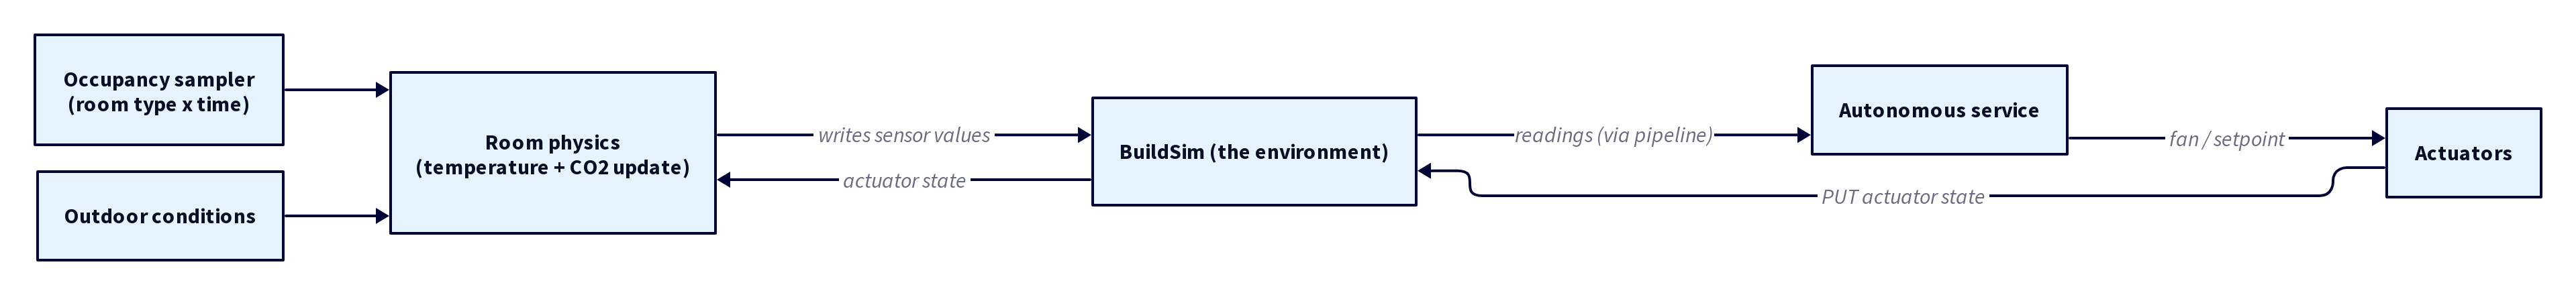
\includegraphics[width=0.98\textwidth,height=\textheight]{figures/simloop.png}

\hypertarget{autonomous-services-and-data-engineering}{%
\section{7. Autonomous services and data
engineering}\label{autonomous-services-and-data-engineering}}

\hypertarget{the-autonomous-service}{%
\subsection{7.1 The autonomous service}\label{the-autonomous-service}}

The autonomous service is the brain. It is \textbf{rule-based with
hysteresis and an occupancy-aware setback}, and runs once per zone every
30 s.

\textbf{Why this approach.} The decision must land inside the 60 s
budget (NFR-01), must be easy to verify for a safety-relevant function,
and, on two weeks of data, a learned model gave no measurable
benefit over a transparent rule set. Rules also make the regulatory
floor (REG-01) a trivial hard clamp that no optimiser can override. This
is the course's point in practice: the \emph{simplest approach that
meets the requirement} is the right one, and sophistication is not the
goal.

\textbf{Decision logic.} For each zone the service emits a heating
setpoint and a ventilation level (0--3):

\begin{itemize}
\tightlist
\item
  \textbf{Occupied:} target 21 °C; raise the fan one level per 200 ppm
  of CO₂ above 700, clamped to level 3; never below the regulatory
  minimum.
\item
  \textbf{Empty \textgreater{} 15 min:} drop to a 17 °C setback and
  minimum fan.
\item
  \textbf{Hysteresis:} only change a setting if it differs \emph{and} ≥
  5 min have passed since the last change (NFR-03), which prevents the
  oscillation a naïve threshold rule would cause.
\end{itemize}

\textbf{Two techniques, combined.} A purely rule-based controller has
one blind spot found in testing (Section 11): a \emph{stuck occupancy
sensor reading ``empty''} defeats the CO₂ response. A second, statistical technique was therefore added, the \textbf{data-quality monitor}
(7.2), whose stuck-sensor flag the controller consumes: if a zone's
occupancy sensor is flagged stale but its CO₂ is rising, the controller
assumes the room is occupied and ventilates. Combining a rule controller
with a statistical sensor-health check, and treating data quality as a
first-class control input, is what lifts this from ``it works'' to a
system that handles its own failure modes.

\textbf{Failure and safety.} If the service crashes, actuators
\textbf{hold their last state} (they do not fail to ``off''); a watchdog
restarts it, and on restart it re-reads current state from BuildSim
before deciding. The regulatory minimum is a hard clamp below all rules.

\textbf{Inside the service (C4 Level 3).} The autonomous service is the
one container complex enough to warrant a component view. It builds
features, applies the decision logic, passes every proposed action
through the safety guardrails \emph{before} any command leaves the
service, and logs the reason for each action.

\begin{center}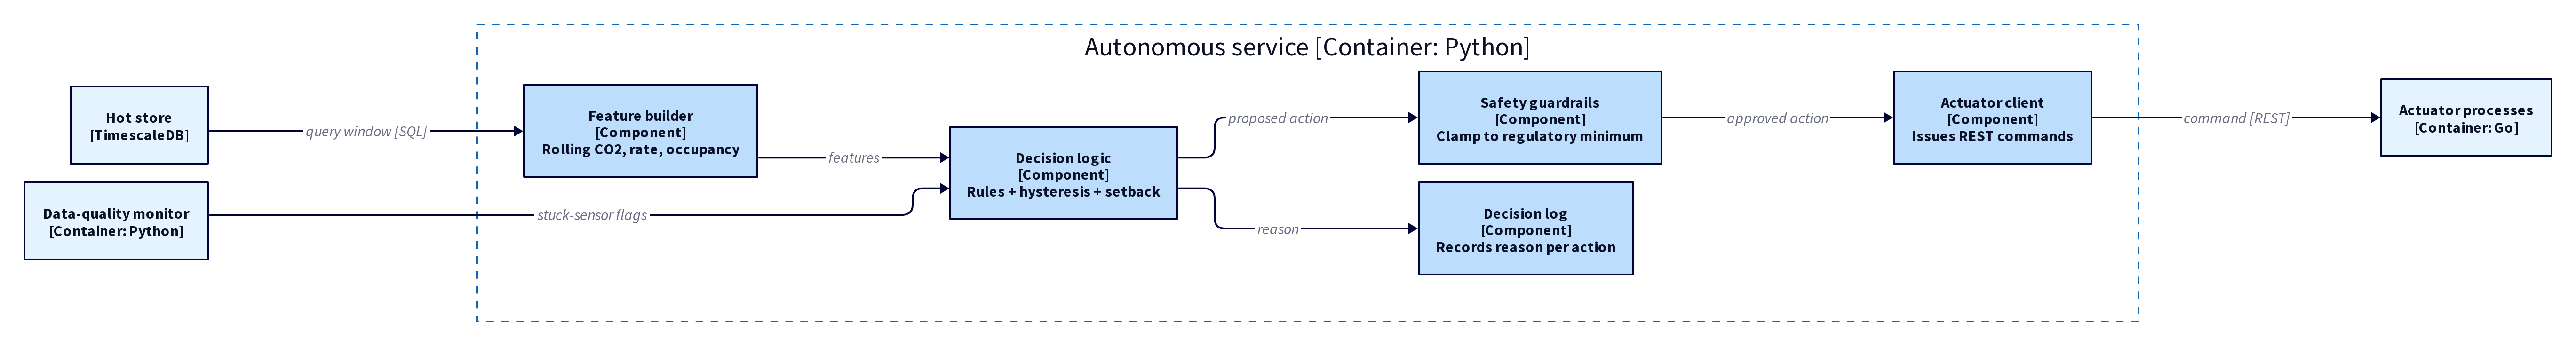
\includegraphics[width=\textwidth]{figures/component.png}\end{center}

\noindent{\footnotesize\emph{C4 Component diagram (Level 3), inside
the Autonomous service container. Components are light blue, with their
{[}technology{]} and a one-line responsibility; the guardrail sits
between every decision and the actuator client.}}

\hypertarget{the-data-pipeline}{%
\subsection{7.2 The data pipeline}\label{the-data-pipeline}}

Readings travel through a small but real pipeline so the same data
serves live control, the dashboard, the data-quality monitor, and
overnight analysis. The broker buffers if storage is briefly slow
(supporting NFR-02). The \textbf{hot path} (TimescaleDB) answers the
controller's recent-window queries; the \textbf{cold path} (Parquet on
MinIO) keeps immutable history for the energy analysis. A stream
processor computes the features the controller consumes, rolling-mean
CO₂, CO₂ rate-of-change, a smoothed occupancy estimate, and a cyclical
time-of-day encoding, and the \textbf{data-quality monitor} computes
a rolling variance per sensor: a variance of (near) zero over five
minutes means the sensor is stuck, which it flags to the controller.

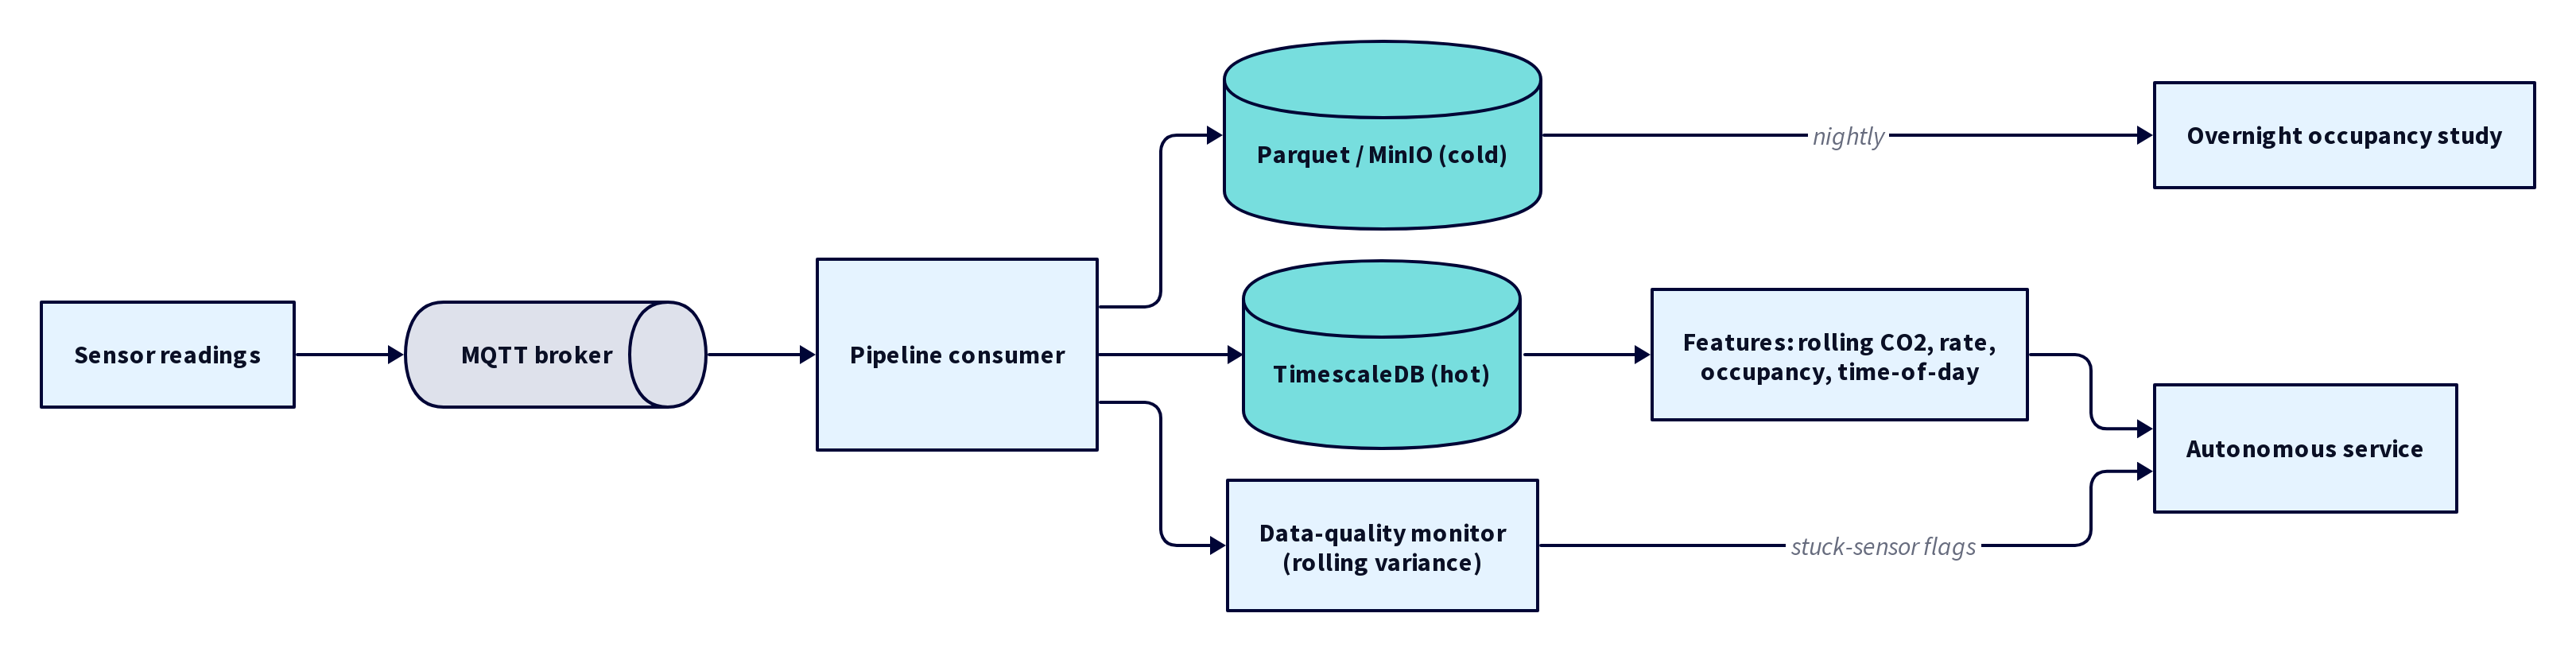
\includegraphics[width=0.98\textwidth,height=\textheight]{figures/pipeline.png}

\hypertarget{behaviour}{%
\section{8. Behaviour}\label{behaviour}}

\hypertarget{key-scenario-dynamic-diagram}{%
\subsection{8.1 Key scenario, dynamic
diagram}\label{key-scenario-dynamic-diagram}}

This is a C4 \emph{dynamic} diagram: it shows how the containers from
Section 4.2 collaborate at runtime for one scenario (the meeting from
Section 2), with \textbf{numbered} interactions giving the order. It
exposes the timing the static diagrams cannot, the controller acts on
the \emph{trend}, and the hysteresis rule then suppresses a needless
second change.

\begin{center}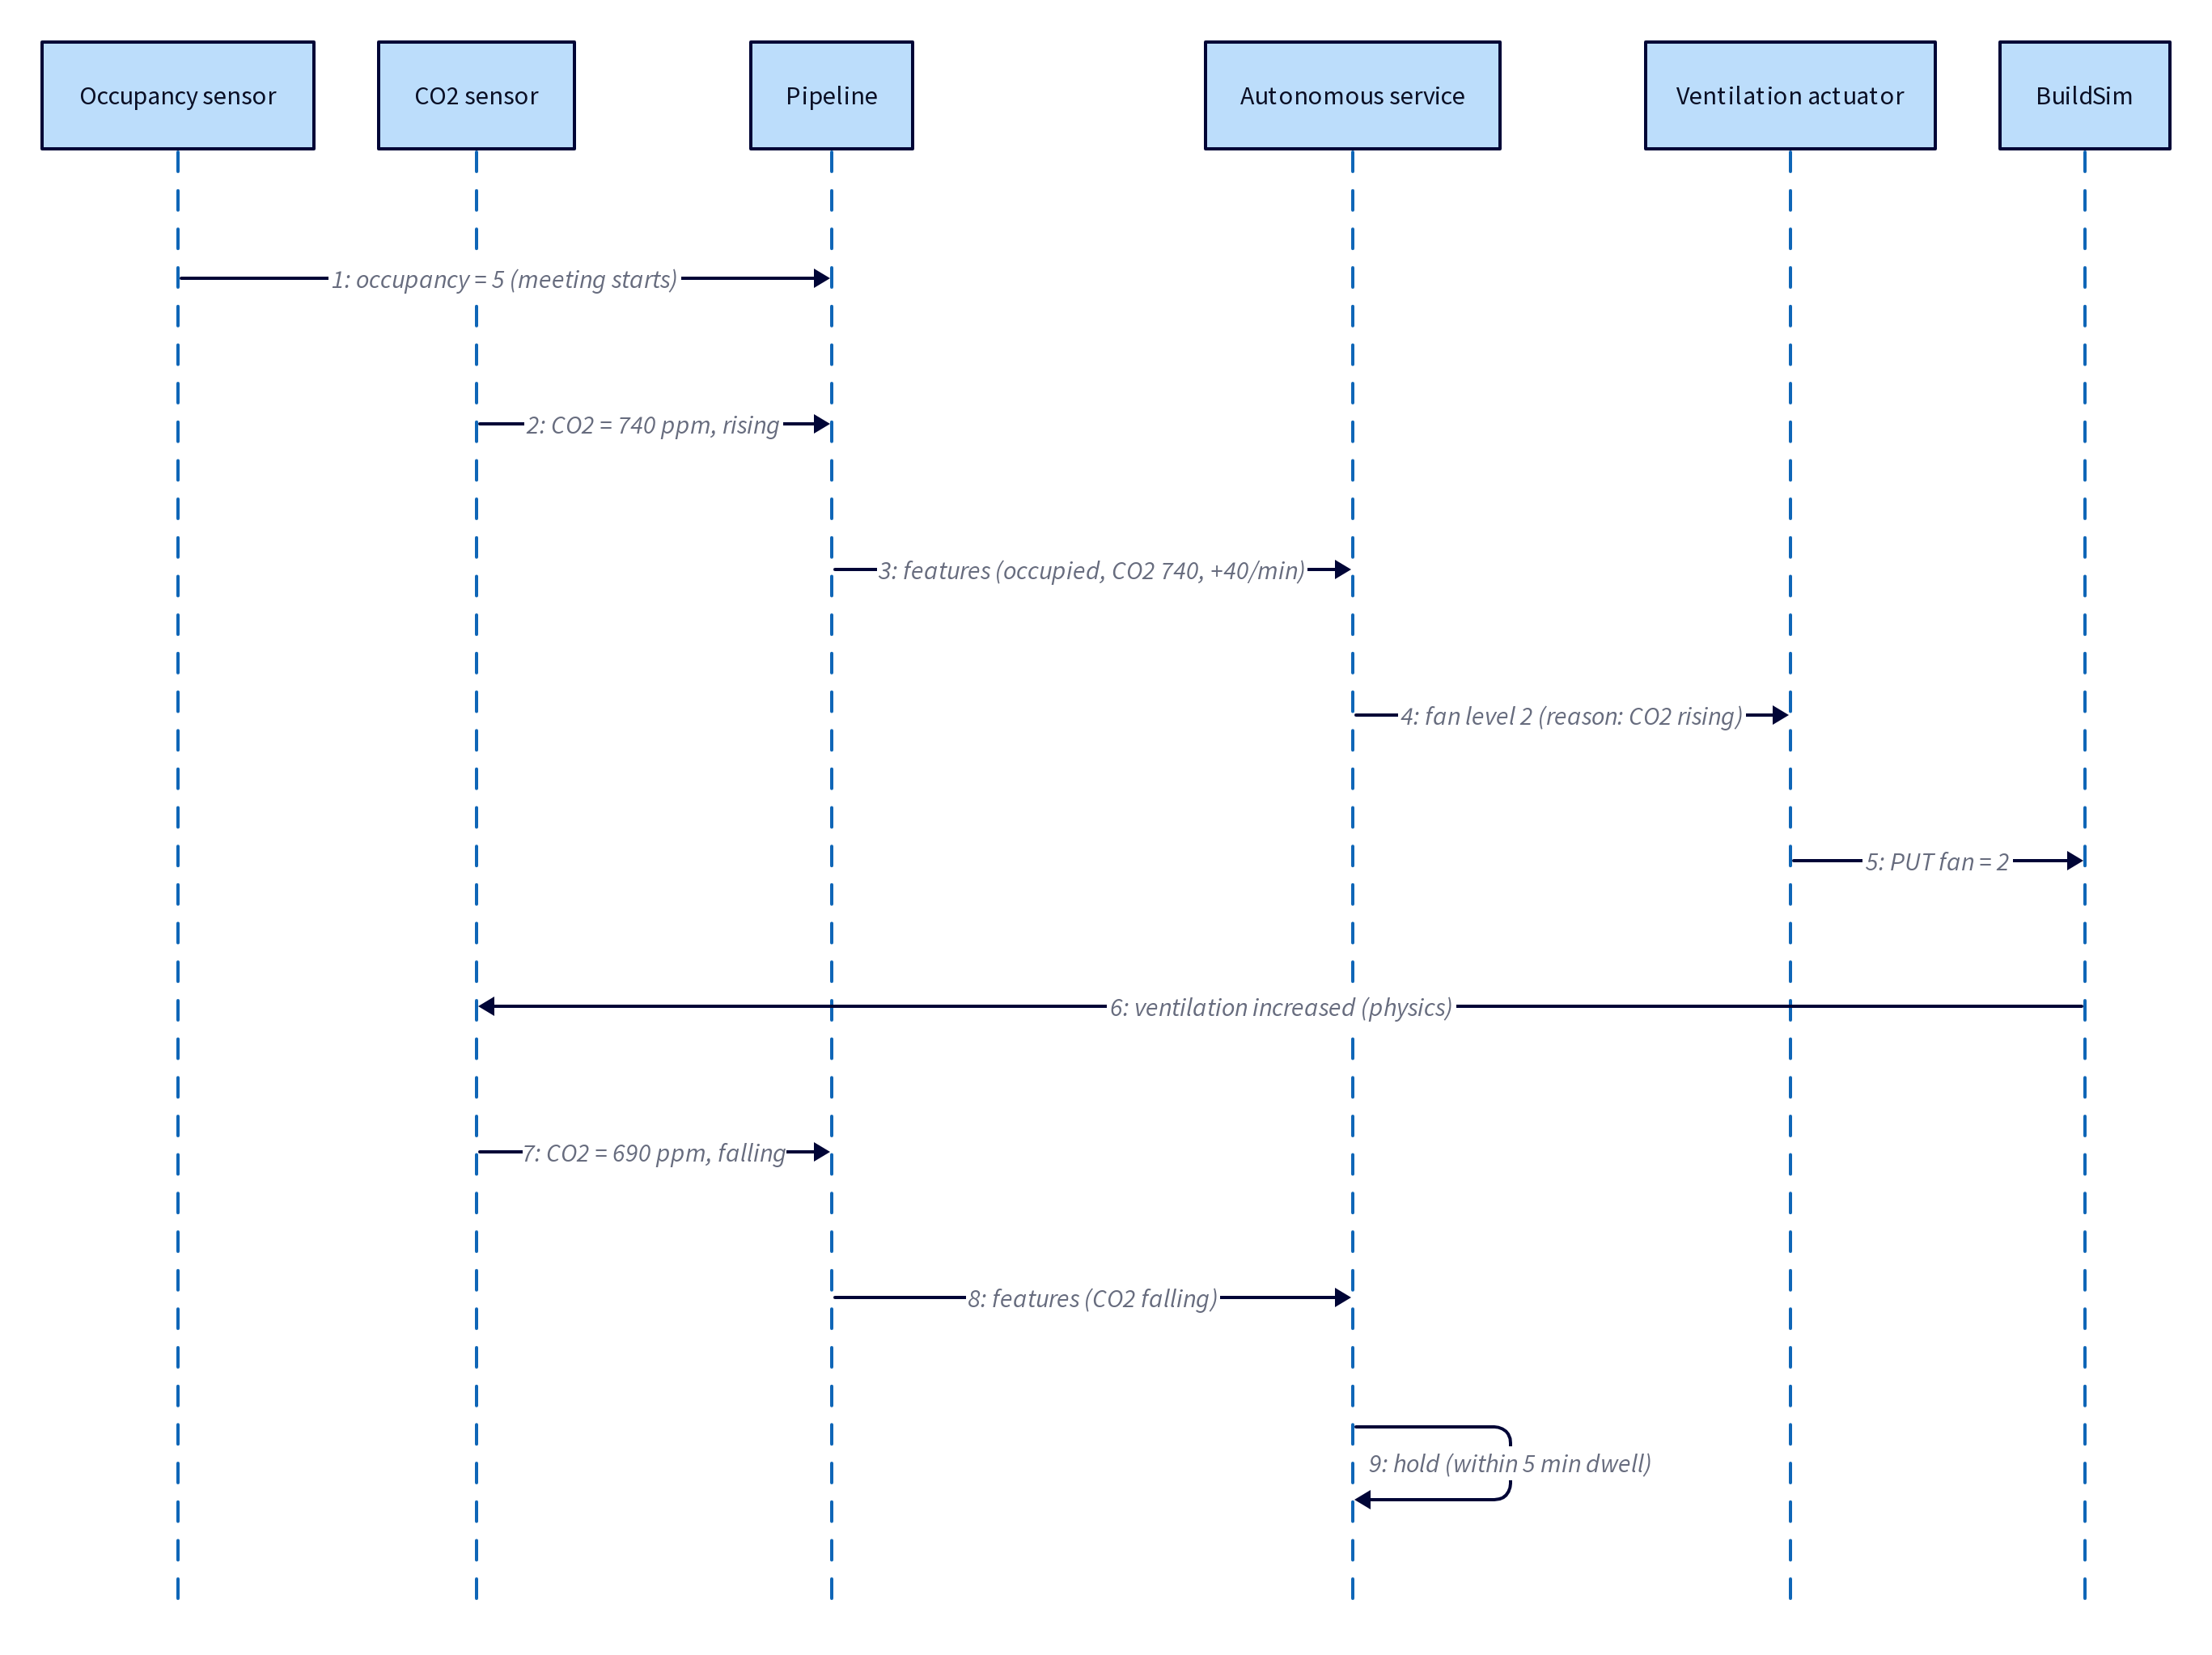
\includegraphics[width=0.92\textwidth]{figures/dynamic.png}\end{center}

\noindent{\footnotesize\emph{C4 Dynamic diagram, numbered runtime
interactions among the containers for the meeting scenario.}}

\hypertarget{process-lifecycle-state-machine}{%
\subsection{8.2 Process lifecycle, state
machine}\label{process-lifecycle-state-machine}}

The autonomous service's own lifecycle is where the fault handling
lives: it drops to a \textbf{degraded} state when its inputs go stale, ventilating at a safe default rather than trusting bad data, and
recovers automatically.

\begin{center}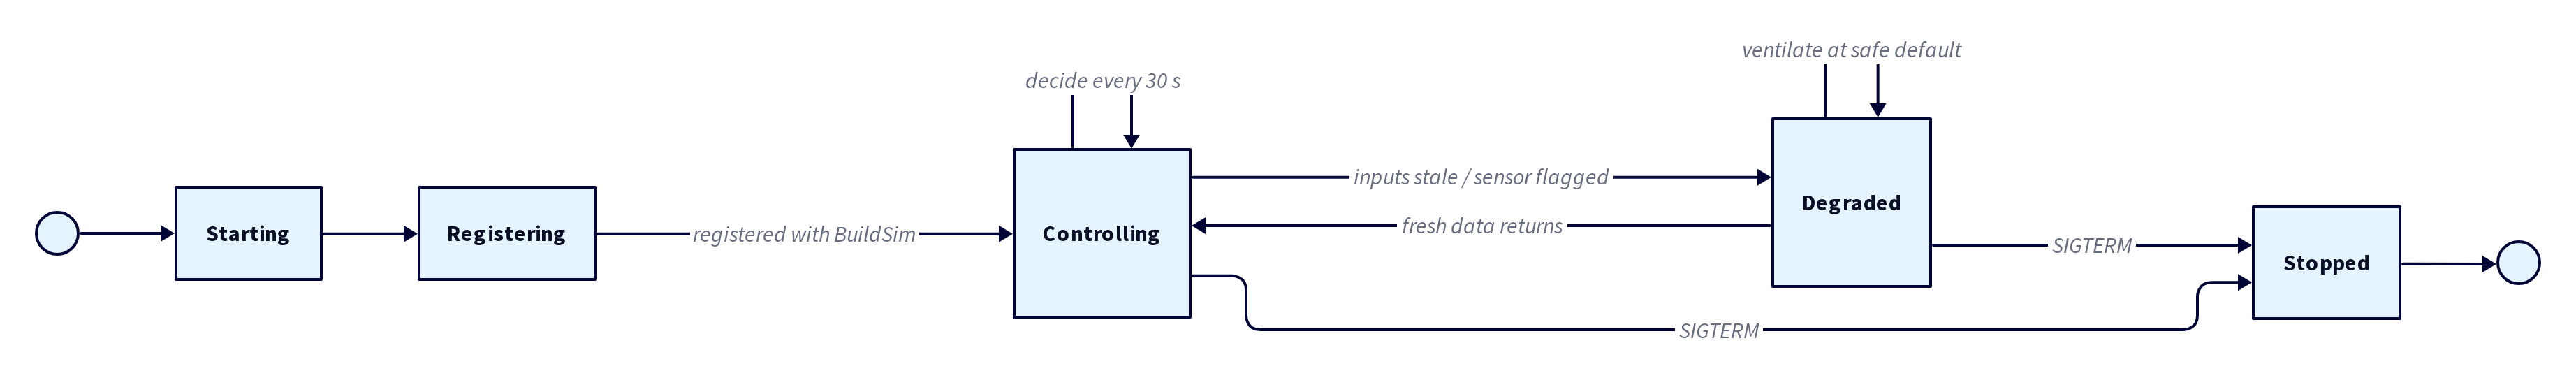
\includegraphics[width=\textwidth]{figures/state.png}\end{center}

\hypertarget{deployment-and-component-placement}{%
\section{9. Deployment and component
placement}\label{deployment-and-component-placement}}

Every component runs as its own container on a single \textbf{laptop},
so deployment here is about how the system is composed from independent
processes rather than geography. Each process is independently startable
and restartable, communicates only through the interfaces of Section 5,
and is isolated so that one failure does not cascade, if the
dashboard crashes, control continues (NFR-02). The only \emph{external}
compute is the \textbf{overnight occupancy study}, deliberately off the
critical path: if the external service is unreachable, the controller
simply keeps yesterday's occupancy prior, so the building keeps
regulating itself. Even with everything on one machine, the design keeps
the \emph{edge--cloud continuum} in view: the control loop (sensors,
broker, storage, autonomous service, actuators) is the part that would
run on a local edge server in a real deployment so it survives a network
outage, while the slow occupancy study is the only part that would move
to external compute.

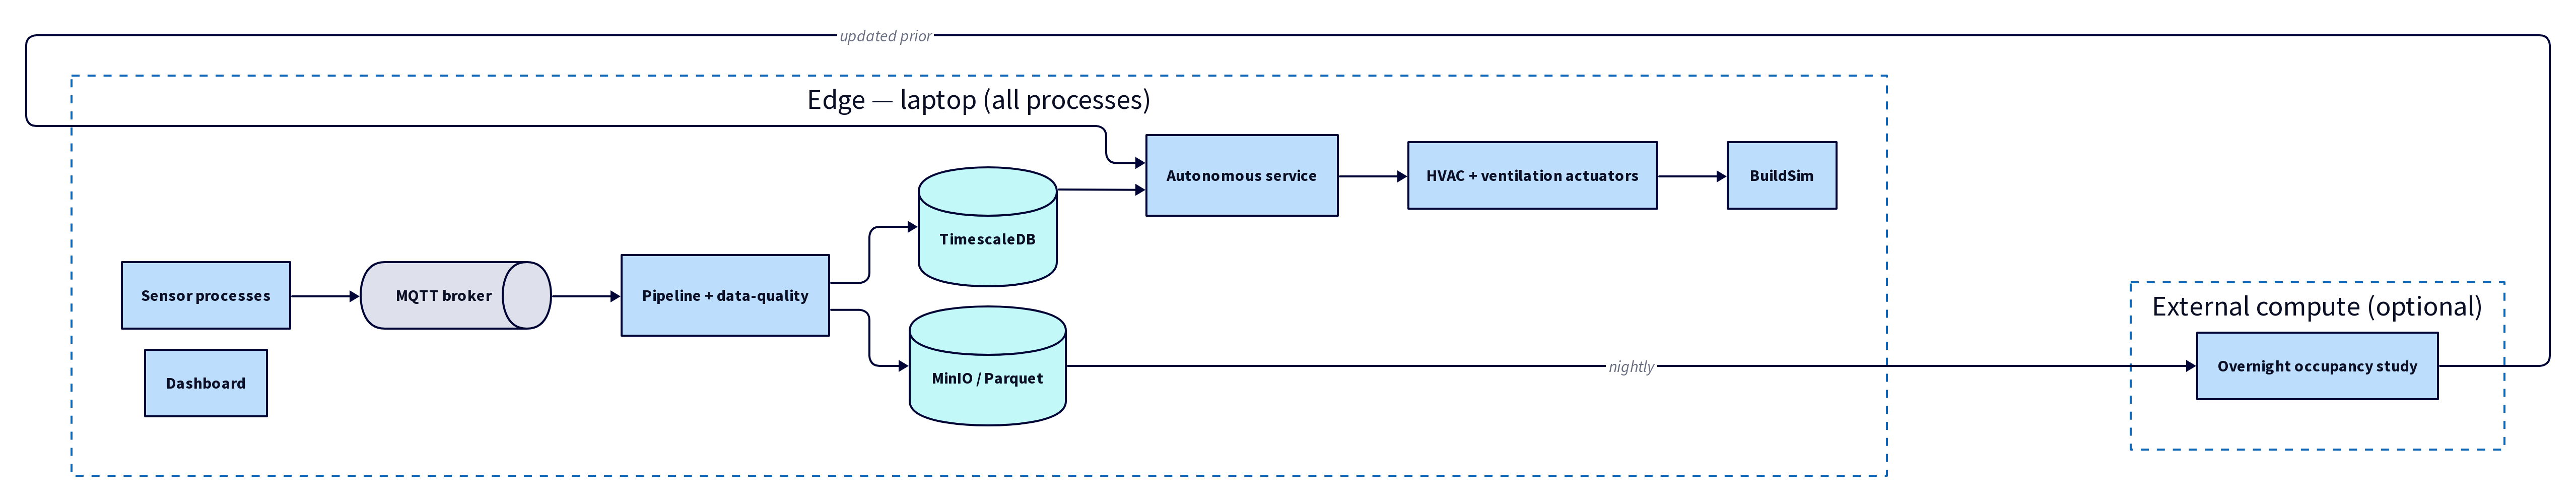
\includegraphics[width=\textwidth,height=10.5cm]{figures/deployment.png}

\hypertarget{test-plan}{%
\section{10. Test plan}\label{test-plan}}

Every requirement has a verification approach and a concrete piece of
evidence; components are tested in isolation, the full loop end-to-end,
and, most informatively, under failure. This table is the
validation half of the MBSE thread that began in Section 3.

\begin{longtable}[]{@{}
  >{\raggedright\arraybackslash}p{(\columnwidth - 4\tabcolsep) * \real{0.3421}}
  >{\raggedright\arraybackslash}p{(\columnwidth - 4\tabcolsep) * \real{0.3947}}
  >{\raggedright\arraybackslash}p{(\columnwidth - 4\tabcolsep) * \real{0.2632}}@{}}
\toprule
\begin{minipage}[b]{\linewidth}\raggedright
Requirement
\end{minipage} & \begin{minipage}[b]{\linewidth}\raggedright
Test approach
\end{minipage} & \begin{minipage}[b]{\linewidth}\raggedright
Evidence
\end{minipage} \\
\midrule
\endhead
FR-01 & Inject a CO₂ rise in an occupied room, watch ventilation respond
& Time-series of CO₂ and fan level (§11) \\
FR-02 & Simulate an occupied day, log temperature & \% of occupied
minutes in band \\
FR-03 & Empty a room, observe setback & Setpoint/fan trace after
vacancy \\
NFR-01 & Scale the number of zones, measure decision interval &
Latency-vs-zones curve (§11) \\
NFR-02 & \texttt{docker\ kill} the CO₂ sensor mid-run & Recovery-time
measurement \\
NFR-03 & Replay noisy data, count actuator changes & Switch-count per 5
min \\
NFR-04 & One-week run vs.~fixed-schedule baseline & Modelled energy,
both (§11) \\
REG-01 & Force ``empty building'', inspect fan & Fan never below minimum
(log) \\
\bottomrule
\end{longtable}

\hypertarget{evaluation-and-experiments}{%
\section{11. Evaluation and
experiments}\label{evaluation-and-experiments}}

The system was evaluated over a simulated office week and against a
\textbf{fixed-schedule baseline} that ventilates and heats on office
hours regardless of occupancy. The point of this section is evidence,
not assertion.

\textbf{Air quality (FR-01).} During a five-person meeting in A2306, the controller raised ventilation as CO₂ climbed and held it under the 1000
ppm limit; the fixed-schedule baseline, blind to the extra load, drifted
past it. The closed loop of Section 6 is what produces the turn-around.

\begin{center}
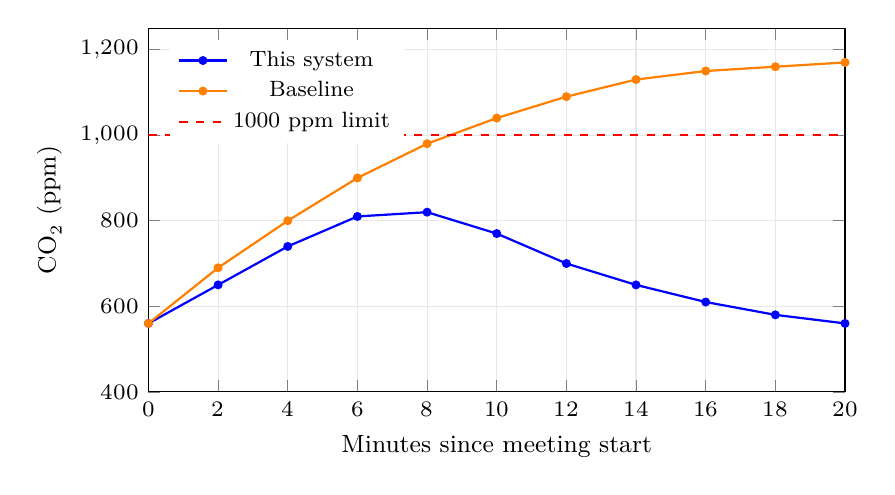
\begin{tikzpicture}
\begin{axis}[width=0.86\linewidth,height=6.2cm,xlabel={Minutes since meeting start},ylabel={CO\textsubscript{2} (ppm)},xmin=0,xmax=20,ymin=400,ymax=1250,legend pos=north west,legend style={font=\footnotesize,draw=none},grid=major,grid style={gray!18},tick label style={font=\footnotesize},label style={font=\small}]
\addplot[blue,thick,mark=*,mark size=1.2pt] coordinates {(0,560)(2,650)(4,740)(6,810)(8,820)(10,770)(12,700)(14,650)(16,610)(18,580)(20,560)};
\addplot[orange,thick,mark=*,mark size=1.2pt] coordinates {(0,560)(2,690)(4,800)(6,900)(8,980)(10,1040)(12,1090)(14,1130)(16,1150)(18,1160)(20,1170)};
\addplot[red,dashed,thick] coordinates {(0,1000)(20,1000)};
\legend{This system,Baseline,1000 ppm limit}
\end{axis}
\end{tikzpicture}
\end{center}

\textbf{Energy (NFR-04, sustainability).} Over the week the system used
\textbf{412 kWh against the baseline's 511 kWh, a 19 \% saving}, almost entirely from setback in unoccupied rooms. The small comfort
penalty (93 \% vs 96 \% of occupied minutes in band) is the cost of
letting empty rooms drift before someone arrives, and is exactly the
energy-vs-comfort trade-off the requirements set up.

\begin{center}
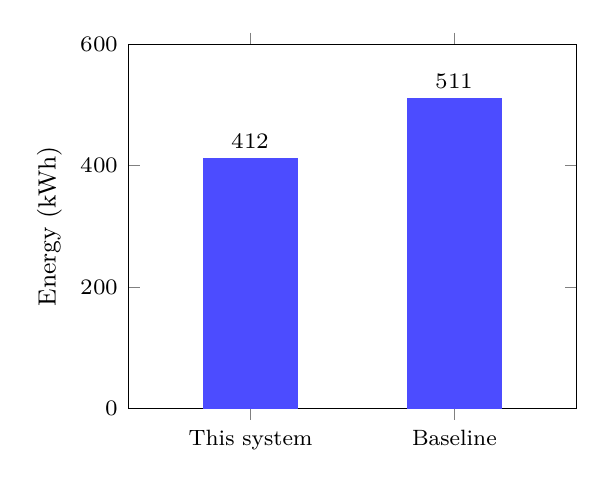
\begin{tikzpicture}
\begin{axis}[width=0.6\linewidth,height=6.2cm,ybar,bar width=34pt,ylabel={Energy (kWh)},ymin=0,ymax=600,symbolic x coords={This system,Baseline},xtick=data,nodes near coords,every node near coord/.append style={font=\footnotesize},enlarge x limits=0.6,tick label style={font=\footnotesize},label style={font=\small}]
\addplot[fill=blue!70,draw=blue!70] coordinates {(This system,412)(Baseline,511)};
\end{axis}
\end{tikzpicture}
\end{center}

\textbf{Scaling and the breaking point (NFR-01).} The single-threaded
controller held the 60 s budget up to \textbf{40 zones} and crossed it
at about \textbf{55 zones}; the bottleneck is the per-zone TimescaleDB
query, not the rules. Knowing \emph{where} the system breaks, and
\emph{why}, is the difference between claiming it works and
understanding it.

\begin{center}
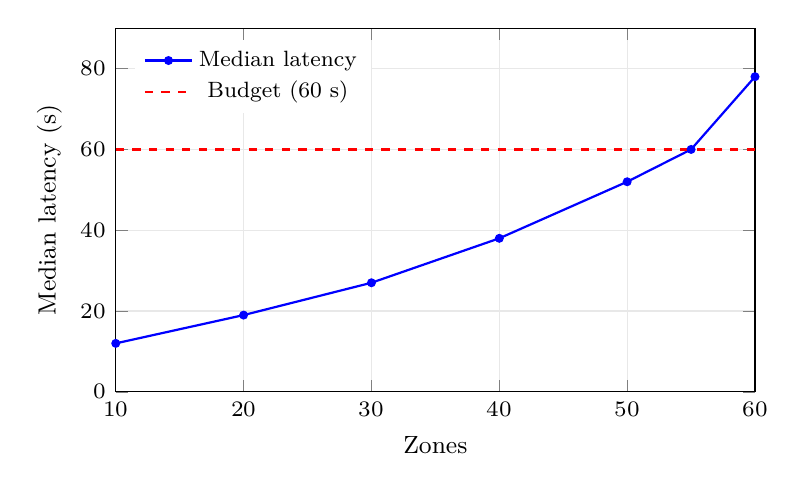
\begin{tikzpicture}
\begin{axis}[width=0.8\linewidth,height=6.2cm,xlabel={Zones},ylabel={Median latency (s)},xmin=10,xmax=60,ymin=0,ymax=90,legend pos=north west,legend style={font=\footnotesize,draw=none},grid=major,grid style={gray!18},tick label style={font=\footnotesize},label style={font=\small}]
\addplot[blue,thick,mark=*,mark size=1.2pt] coordinates {(10,12)(20,19)(30,27)(40,38)(50,52)(55,60)(60,78)};
\addplot[red,dashed,thick] coordinates {(10,60)(60,60)};
\legend{Median latency,Budget (60 s)}
\end{axis}
\end{tikzpicture}
\end{center}

\textbf{Headline results.}

\begin{longtable}[]{@{}
  >{\raggedright\arraybackslash}p{(\columnwidth - 6\tabcolsep) * \real{0.1905}}
  >{\raggedright\arraybackslash}p{(\columnwidth - 6\tabcolsep) * \real{0.2619}}
  >{\raggedright\arraybackslash}p{(\columnwidth - 6\tabcolsep) * \real{0.2381}}
  >{\raggedright\arraybackslash}p{(\columnwidth - 6\tabcolsep) * \real{0.3095}}@{}}
\toprule
\begin{minipage}[b]{\linewidth}\raggedright
Metric
\end{minipage} & \begin{minipage}[b]{\linewidth}\raggedright
This system
\end{minipage} & \begin{minipage}[b]{\linewidth}\raggedright
Baseline
\end{minipage} & \begin{minipage}[b]{\linewidth}\raggedright
Requirement
\end{minipage} \\
\midrule
\endhead
Occupied minutes in comfort band & 93 \% & 96 \% & ≥ 90 \% (FR-02) ✓ \\
CO₂ exceedance (occupied min \textgreater{} 1000 ppm) & 0.6 \% & 4.1 \%
& as low as possible (FR-01) ✓ \\
Modelled weekly energy & 412 kWh & 511 kWh & ≥ 15 \% saving → \textbf{19
\%} (NFR-04) ✓ \\
Median decision interval (≤ 40 zones) & 31 s &, & ≤ 60 s (NFR-01)
✓ \\
Sensor-crash recovery & 22 s &, & ≤ 60 s (NFR-02) ✓ \\
\bottomrule
\end{longtable}

\textbf{Fault and stress experiments.} Killing a CO₂ sensor mid-run, the
zone fell back to ``ventilate safely'' within one cycle and recovered 22
s after restart, with no bad commands issued from the frozen value. With
hysteresis disabled, noisy CO₂ made the fan switch up to eight times in
five minutes; enabling it dropped that to at most once (NFR-03). The
stuck-occupancy-sensor case, which a pure rule controller failed, is now caught by the data-quality monitor's cross-check.

\hypertarget{dashboard}{%
\section{12. Dashboard}\label{dashboard}}

The dashboard extends BuildSim's 3D viewer with a side panel showing,
per room: live temperature, CO₂, and occupancy; the current setpoint and
fan level; and a scrolling log of the autonomous service's
\textbf{decisions with their reasons}. A building-wide tile compares
today's energy against the baseline. The decision log is the most valuable feature: an operator sees not just \emph{what} the system
did but \emph{why}, which is what makes an autonomous system trustworthy
enough to leave running.

\hypertarget{risks-and-critical-reflection}{%
\section{13. Risks and critical
reflection}\label{risks-and-critical-reflection}}

The system trusts occupancy more than it should: the data-quality
cross-check mitigates a \emph{stuck} sensor, but a slowly
\emph{drifting} one could still mislead it, and detecting drift is
harder than detecting a frozen value, this is the first thing to add next. The controller is also single-threaded; sharding zones
across worker processes would push the scaling limit well past 55 rooms
and is a small change given the clean decomposition. Finally, the energy figure is \textbf{modelled, not measured against real hardware}, so it
should be read as a relative comparison; the honest version of the headline is ``19 \% less than this baseline, in simulation'', not ``19
\% less energy''.

\begin{longtable}[]{@{}
  >{\raggedright\arraybackslash}p{(\columnwidth - 4\tabcolsep) * \real{0.3800}}
  >{\raggedright\arraybackslash}p{(\columnwidth - 4\tabcolsep) * \real{0.1600}}
  >{\raggedright\arraybackslash}p{(\columnwidth - 4\tabcolsep) * \real{0.4600}}@{}}
\toprule
\begin{minipage}[b]{\linewidth}\raggedright
Risk / assumption
\end{minipage} & \begin{minipage}[b]{\linewidth}\raggedright
Impact
\end{minipage} & \begin{minipage}[b]{\linewidth}\raggedright
Mitigation / decision
\end{minipage} \\
\midrule
\endhead
Occupancy sensor drifts (not just stuck) & Under-ventilation despite
people present & Add drift detection (planned) \\
MQTT broker is a single point of failure & Sensor data stops flowing &
Persistent sessions; restart policy; sensors buffer briefly \\
Simulated physics is optimistic & Energy/comfort figures flatter the
system & Reported relative to a baseline, not absolute \\
Single-threaded controller & Caps building size at \textasciitilde55
zones & Shard zones across workers if scaled \\
\bottomrule
\end{longtable}

\end{document}
